% !TEX TS-program = xelatex
% !TEX encoding = UTF-8 Unicode
% -*- coding: UTF-8; -*-
% vim: set fenc=utf-8

%%%%%%%%%%%%%%%%%%%%%%%%%%%%%%%%%%%%%%%%%%%%%%%%%%%%%%%%%%%%%%%%%
%% SIMPLE-THESIS-DISSERTATION
%% <https://github.com/zachscrivena/simple-thesis-dissertation>
%% This is free and unencumbered software released into the
%% public domain; see <http://unlicense.org> for details.
%%%%%%%%%%%%%%%%%%%%%%%%%%%%%%%%%%%%%%%%%%%%%%%%%%%%%%%%%%%%%%%%%

% See "README.md" for instructions on compiling this document.

\documentclass[letterpaper,nonstop,draftmode]{simplethesisdissertation}
% Class options:
% a4paper, letterpaper, nonstop, draftmode.

%%%%%%%%%%%%%%%%%%%%%%%%%%%%%%%%%%%%%%%%%%%%%%%%%%%%%%%%%%%%%%%%%
%% PREAMBLE.
%%%%%%%%%%%%%%%%%%%%%%%%%%%%%%%%%%%%%%%%%%%%%%%%%%%%%%%%%%%%%%%%%

% Document properties.
\def\DocumentTitle{Hardware Accelerated List Decoding and Simulation}
\def\AuthorName{Joshua Mathew}

% PDF settings and properties.
\hypersetup{
pdftitle={\DocumentTitle},
pdfauthor={\AuthorName},
pdfsubject={Undergraduate Thesis, University of California Los Angeles, 2023},
pdfcreator={XeLaTeX},
pdfproducer={},
pdfkeywords={},
unicode=true,
bookmarks=true,
bookmarksopen=true,
pdfstartview=FitH,
pdfpagelayout=OneColumn,
pdfpagemode=UseOutlines,
hidelinks,
breaklinks,
bookmarksnumbered}

% Accent colors.
\definecolor{AccentOne}{RGB}{0,68,186} % blue

% Macros:
\DeclareMathOperator*{\argmax}{arg\,max}
\DeclareMathOperator*{\argmin}{arg\,min}
\renewcommand{\binom}[2]{\left(\genfrac{}{}{0pt}{}{#1}{#2}\right)}
\newcommand{\ceil}[1]{{\left\lceil{#1}\right\rceil}}
%\newcommand{\ffrac}[2]{{\nicefrac{#1}{#2}}}
%\newcommand{\fffrac}[2]{{\left.{#1}\middle/{#2}\right.}}
\newcommand{\floor}[1]{{\left\lfloor{#1}\right\rfloor}}
\DeclareMathOperator{\lcm}{lcm}
\newcommand{\ZZ}{{\mathbb{Z}}}

%%%%%%%%%%%%%%%%%%%%%%%%%%%%%%%%%%%%%%%%%%%%%%%%%%%%%%%%%%%%%%%%%
%% ACTUAL DOCUMENT.
%%%%%%%%%%%%%%%%%%%%%%%%%%%%%%%%%%%%%%%%%%%%%%%%%%%%%%%%%%%%%%%%%

\begin{document}

% Use Roman numerals (i, ii, iii, etc.) for page numbers in the front matter.
\pagenumbering{roman}

%%%%%%%%%%%%%%%%%%%%%%%%%%%%%%%%%%%%%%%%%%%%%%%%%%%%%%%%%%%%%%%%%
%% TITLE PAGE.
%%%%%%%%%%%%%%%%%%%%%%%%%%%%%%%%%%%%%%%%%%%%%%%%%%%%%%%%%%%%%%%%%

% No headers or footers on the title page.
\thispagestyle{empty}

\begingroup
\centering
\setstretch{1.0}
~
\\[1em]
\sffamily\bfseries\fontsize{26}{31.2}\selectfont
\DocumentTitle
\\[0.4in]
\normalfont\large
Thesis by
\\[0.25em]
\sffamily\bfseries\Large
\AuthorName
\\[0.4in]
\normalfont\normalsize
In Partial Fulfillment of the Requirements
\\[0.5em]
for the Degree of
\\[0.5em]
Bachelors of Science
\\[0.5em]
in
\\[0.5em]
Electrical Engineering 
\vfill

\includegraphics[width=1.8in]
{Figures/UCLA_logo.png}
\\[1.5em]
University California, Los Angeles
\\[0.5em]
Los Angeles, California, USA
\\[1.5em]
2023
\\[0.5em]
\par
\endgroup

\clearpage

%%%%%%%%%%%%%%%%%%%%%%%%%%%%%%%%%%%%%%%%%%%%%%%%%%%%%%%%%%%%%%%%%
%% COPYRIGHT PAGE.
%%%%%%%%%%%%%%%%%%%%%%%%%%%%%%%%%%%%%%%%%%%%%%%%%%%%%%%%%%%%%%%%%

\pagestyle{plain}
\setcounter{page}{2}

\begingroup
\centering
\setstretch{1.0}
\null
\vfill
{\sffamily\textcopyright}~2023
\\[0.5em]
\AuthorName
\\[0.5em]
All Rights Reserved
\par
\endgroup

\clearpage

%%%%%%%%%%%%%%%%%%%%%%%%%%%%%%%%%%%%%%%%%%%%%%%%%%%%%%%%%%%%%%%%%
%% DEDICATION PAGE.
%%%%%%%%%%%%%%%%%%%%%%%%%%%%%%%%%%%%%%%%%%%%%%%%%%%%%%%%%%%%%%%%%

%\begingroup
%\centering
%\setstretch{1.0}
%~
%\\[1in]
%\textit{Insert dedication here}
%\par
%\endgroup

%\clearpage

%%%%%%%%%%%%%%%%%%%%%%%%%%%%%%%%%%%%%%%%%%%%%%%%%%%%%%%%%%%%%%%%%
%% ACKNOWLEDGMENTS.
%%%%%%%%%%%%%%%%%%%%%%%%%%%%%%%%%%%%%%%%%%%%%%%%%%%%%%%%%%%%%%%%%

\chapter*{Acknowledgments}
\addcontentsline{toc}{chapter}{Acknowledgments}

I would like to dedicate this section of the thesis to acknowledging the contributions of my supervisors, predecessors, and peers that made this work possible. I thank Professor Richard Wesel for introducing me to and supporting me through the list decoding and noise generation projects. He has also been an amazing source of mentorship providing me with technical understanding of coding theory where I lacked it and a role model for leading, collaborating with, and communicating with a diverse team. Furthermore, I would like to thank Caleb Terril and Chester Hulse for being amazing mentors in this lab. Their work has been the foundation for which the work presented in this paper adds to. Lastly I would like to thank my peers Aadhirahvi Ravikumar, Daniel Chen, and the rest of the CSL undergraduates that have contributed to this project and its adjacent ones. 

\clearpage

%%%%%%%%%%%%%%%%%%%%%%%%%%%%%%%%%%%%%%%%%%%%%%%%%%%%%%%%%%%%%%%%%
%% ABSTRACT.
%%%%%%%%%%%%%%%%%%%%%%%%%%%%%%%%%%%%%%%%%%%%%%%%%%%%%%%%%%%%%%%%%

\chapter*{Abstract}
\addcontentsline{toc}{chapter}{Abstract}

Efficient, lossless data transmission has proven integral to the functioning of modern society. Short block length codes, more specifically convolutional codes, have provided ultra reliable low latency performance in applications such as cellular and satellite communications. Furthermore, CRC-aided, tail-biting convolutional codes have shown to approach the RCU bound with a large number of states. Serial List Viterbi Decoding (SLVD) and Parallel List Viterbi Decoding (PLVD) are methods of decoding these codes that approximate Maximum-Likelihood (ML) as the list size increases. This thesis will overview an implementation of PLVD on a field-programmable gate array (FPGA) board as well as justify the algorithmic advantages of PLVD for hardware acceleration. This design has been heavily inspired by the work of Chester Hulse, former member of CSL, and this paper will illustrate that the modifications result in a more resource efficient implementation of his work. These changes have made room for more hardware accelerated modules such as an additive white gaussian noise (AWGN) generator on board. This thesis will also briefly introduce an implementation of this in hardware.

\clearpage

%%%%%%%%%%%%%%%%%%%%%%%%%%%%%%%%%%%%%%%%%%%%%%%%%%%%%%%%%%%%%%%%%
%% TABLE OF CONTENTS (TOC), LISTS OF FIGURES, TABLES, ETC.
%%%%%%%%%%%%%%%%%%%%%%%%%%%%%%%%%%%%%%%%%%%%%%%%%%%%%%%%%%%%%%%%%

\tableofcontents

\listoffigures

\listoftables

\clearpage

% Use Arabic numerals (1, 2, 3, etc.) for subsequent page numbers.
\pagenumbering{arabic}


\chapter{Introduction}
Information communication has become an integral part of the fabric of our society, influencing how we connect, learn, work, and interact with one another. Advancements in data transmission and standardized communications protocols have transformed the way we communicate and exchange information. They enable us to bridge geographical boundaries, maintaining relationships and forming new connections across the globe. Furthermore, they play a pivotal role in business and commerce, enabling seamless collaboration, efficient transactions, and global market access. And lastly, communication systems facilitate civic engagement, empowering individuals to voice their opinions, participate in political processes, and advocate for social change.

An important application of information communication is the data sent for control and usage of sensors, peripheral devices, and processing nodes. Communication protocols for these purposes often involve the use of short length messages and a convolutional coding scheme aided by a Cyclic Redundancy Check (CRC). This coding scheme is used in modern cell phone standards \cite{ETSI_conf} and even space communication systems \cite{Space_appl}. Furthermore, adding a tail biting condition (TB) for frame synchronization has shown to approach the RCU bound with a large number of states \cite{coskun}. 

This project aims to implement a scalable list decoder on an FPGA that can provide a maximum likelihood decoding of CRC aided tail biting convolutional codes (TBCC). We also introduce a hardware implementation of a additive white gaussian noise (AWGN) generator for accelerating end to end simulation of code performance.



\chapter{Background}

\section{Convolutional Encoding}

Convolutional Codes are a type of error correcting code (ECC) that use memory storing elements and convolution of a message with a generator polynomial to encode each transmitted bit. In this chapter we use the notion described in \Table~\tref{Table:Background:SymbolDefinitions}.

%%%%%%%%%%%%%%%%%%%%%%%%%%%%%%%%%%%%%%%%%%%%%%%%%%%%%%%%%%%%%%%%%
% TABLE: BACKGROUND: Symbol Definitions
\begin{table}
\caption[Background chapter symbols and definitions]
{Background chapter symbols and definitions}
\label{Table:Background:SymbolDefinitions}
\centering\CaptionFontSize
\begin{tabular}{c@{\hspace{1em}}l}
\toprule
Symbol & Definition
\\
\midrule
$N$ & number of memory storing elements (number of bits in a state)
\\
$T$ & length of pre-encoded message in bits
\\
$k$ & rate of the encoder (1/k); we use a rate 1/5 (k=5) encoder in our simulations
\\

\bottomrule
\end{tabular}
\end{table}
%%%%%%%%%%%%%%%%%%%%%%%%%%%%%%%%%%%%%%%%%%%%%%%%%%%%%%%%%%%%%%%%%

\subsection{Generator Polynomial and Convolution}

At a basic level, Convolutional Codes encode a message by performing a discrete time convolution on a stream of message bits. This is done by storing the N previous bits streamed and then performing a series of XORs operations with them and the next bit to result in an encoding. The series of XORs (1-bit XOR is equivalent to addition) performed defines the generator polynomial that we are convolving with the pre-encoded message. An example of this is shown in \Figure~\fref{Figure:Background:ConvolutionalEncoderArchitecture}. 

%%%%%%%%%%%%%%%%%%%%%%%%%%%%%%%%%%%%%%%%%%%%%%%%%%%%%%%%%%%%%%%%%
% FIGURE: BACKGROUND: Convolutional Encoder Architecture
\begin{figure}
\centering\CaptionFontSize
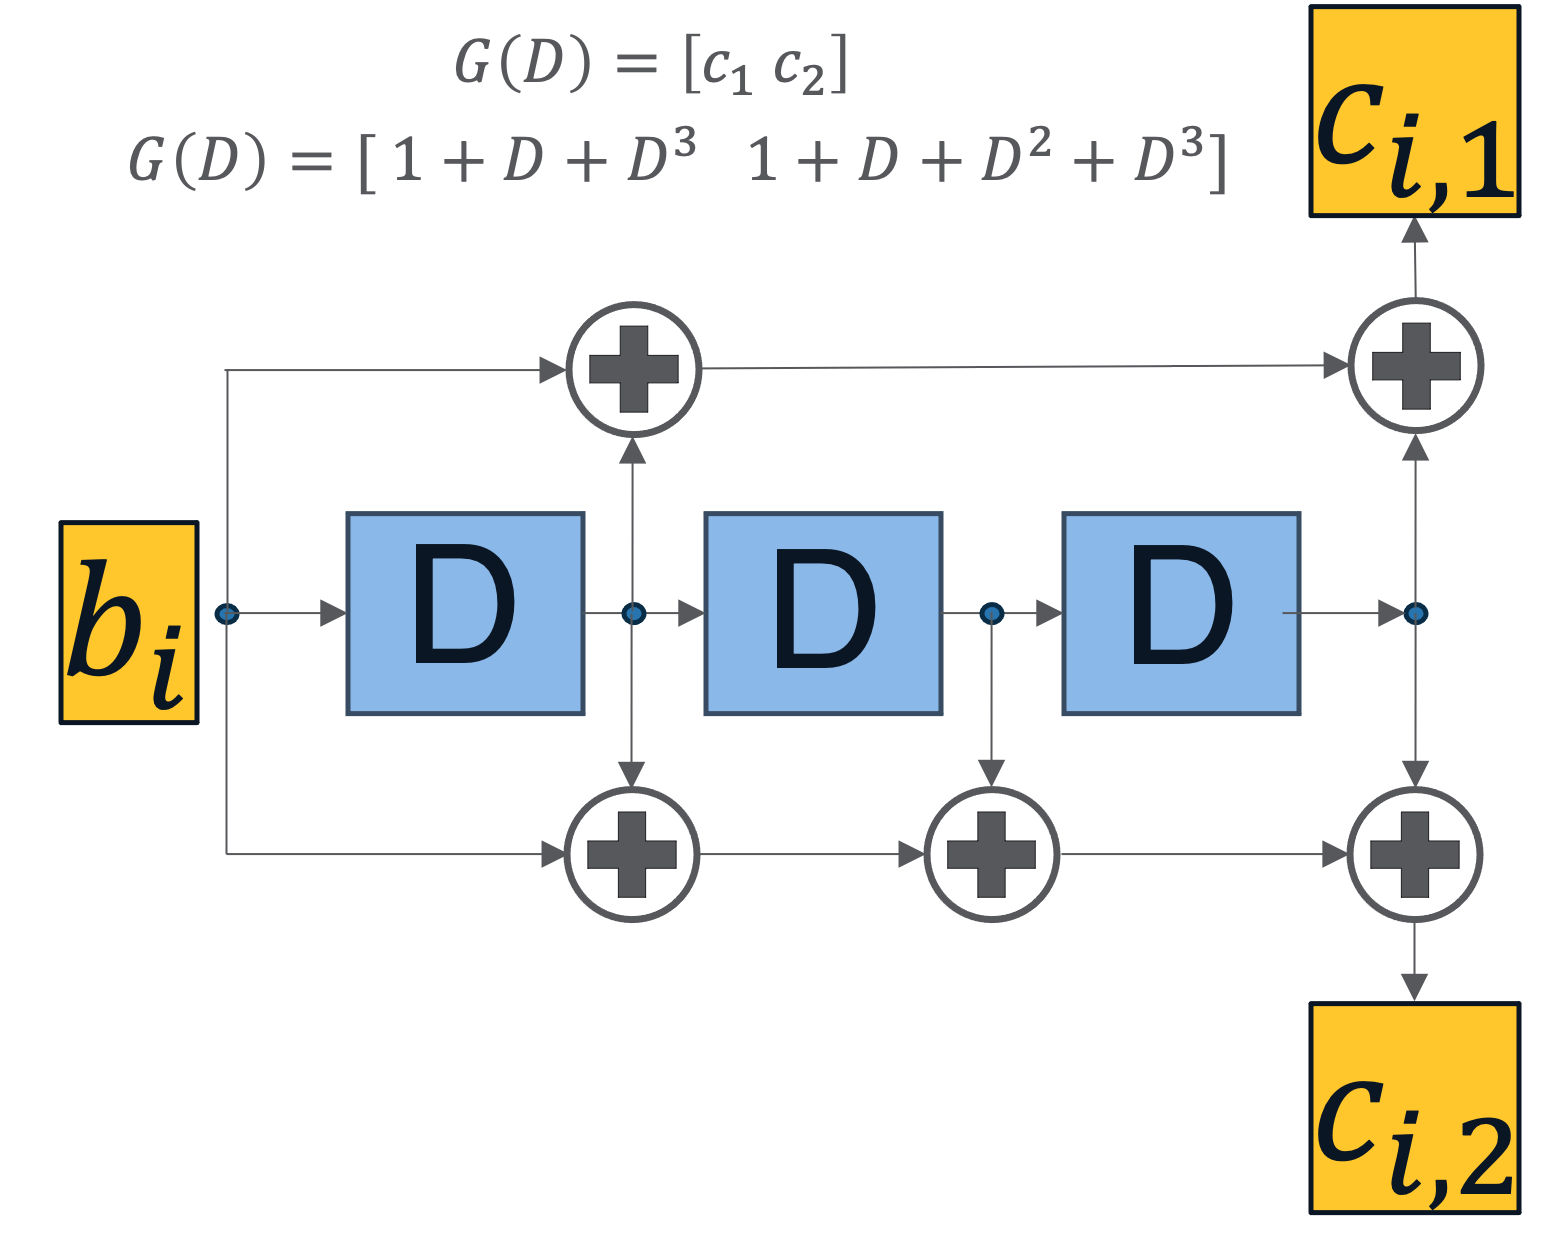
\includegraphics[height=15em]
{Figures/convolutional_encoding_hw.png}
\caption[Implementation of a convolutional encoder with a given generator polynomial]
{Implementation of a convolutional encoder with a given generator polynomial}
\label{Figure:Background:ConvolutionalEncoderArchitecture}
\end{figure}
%%%%%%%%%%%%%%%%%%%%%%%%%%%%%%%%%%%%%%%%%%%%%%%%%%%%%%%%%%%%%%%%%

Here $(u_n)$ is the sequence of bits being streamed and $c_{1,i}$ and $c_{2,i}$ correspond to the (in this example) two bit encoding of $u_i$. Furthermore, each memory storing element $D$ is cascaded and will store and output the last value that was at its input. Thus, based on the above architecture, each $u_i$ is encoded to $[c_{1,i} \quad c_{2,i}]$ where 
$$[c_{1,i} \quad c_{2,i}] = [ u_i + u_{i-1} + u_{i-3} \quad u_i + u_{i+1} + u_{i+2} + u_i]$$

In other words, the sequence $c = [(c_1,n)  \quad (c_2,n) ]$ is a discrete convolution of $(u_n)$ with the sequence $(g_n) =  [ [1  1 0 1] \quad [1 1 1 1]]$. In the polynomial representation, $c(D) = u(D)G(D)$, the generator polynomial that then represents this specific encoding would be 
$$G(D) =	[1 + D + D^3  \quad 1+ D + D^2 + D^3]$$

It is worth noting that the output of the encoder will output the sequence $c$ in the following format
$$c = (c_{1,0}, c_{2,0}, c_{1,1}, c_{2,1}, \ldots, c_{1,i}, c_{2,i}, \ldots, c_{1,T}, c_{2,T})$$

\subsection{State Diagram Representation}
A useful interpretation of the encoding process is as transitions in a state diagram as shown in \Figure~\fref{Figure:Background:ConvolutionalCodeStateDiagram}.

%%%%%%%%%%%%%%%%%%%%%%%%%%%%%%%%%%%%%%%%%%%%%%%%%%%%%%%%%%%%%%%%%
% FIGURE: BACKGROUND: Convolutional Encoder State Diagram
\begin{figure}
\centering\CaptionFontSize
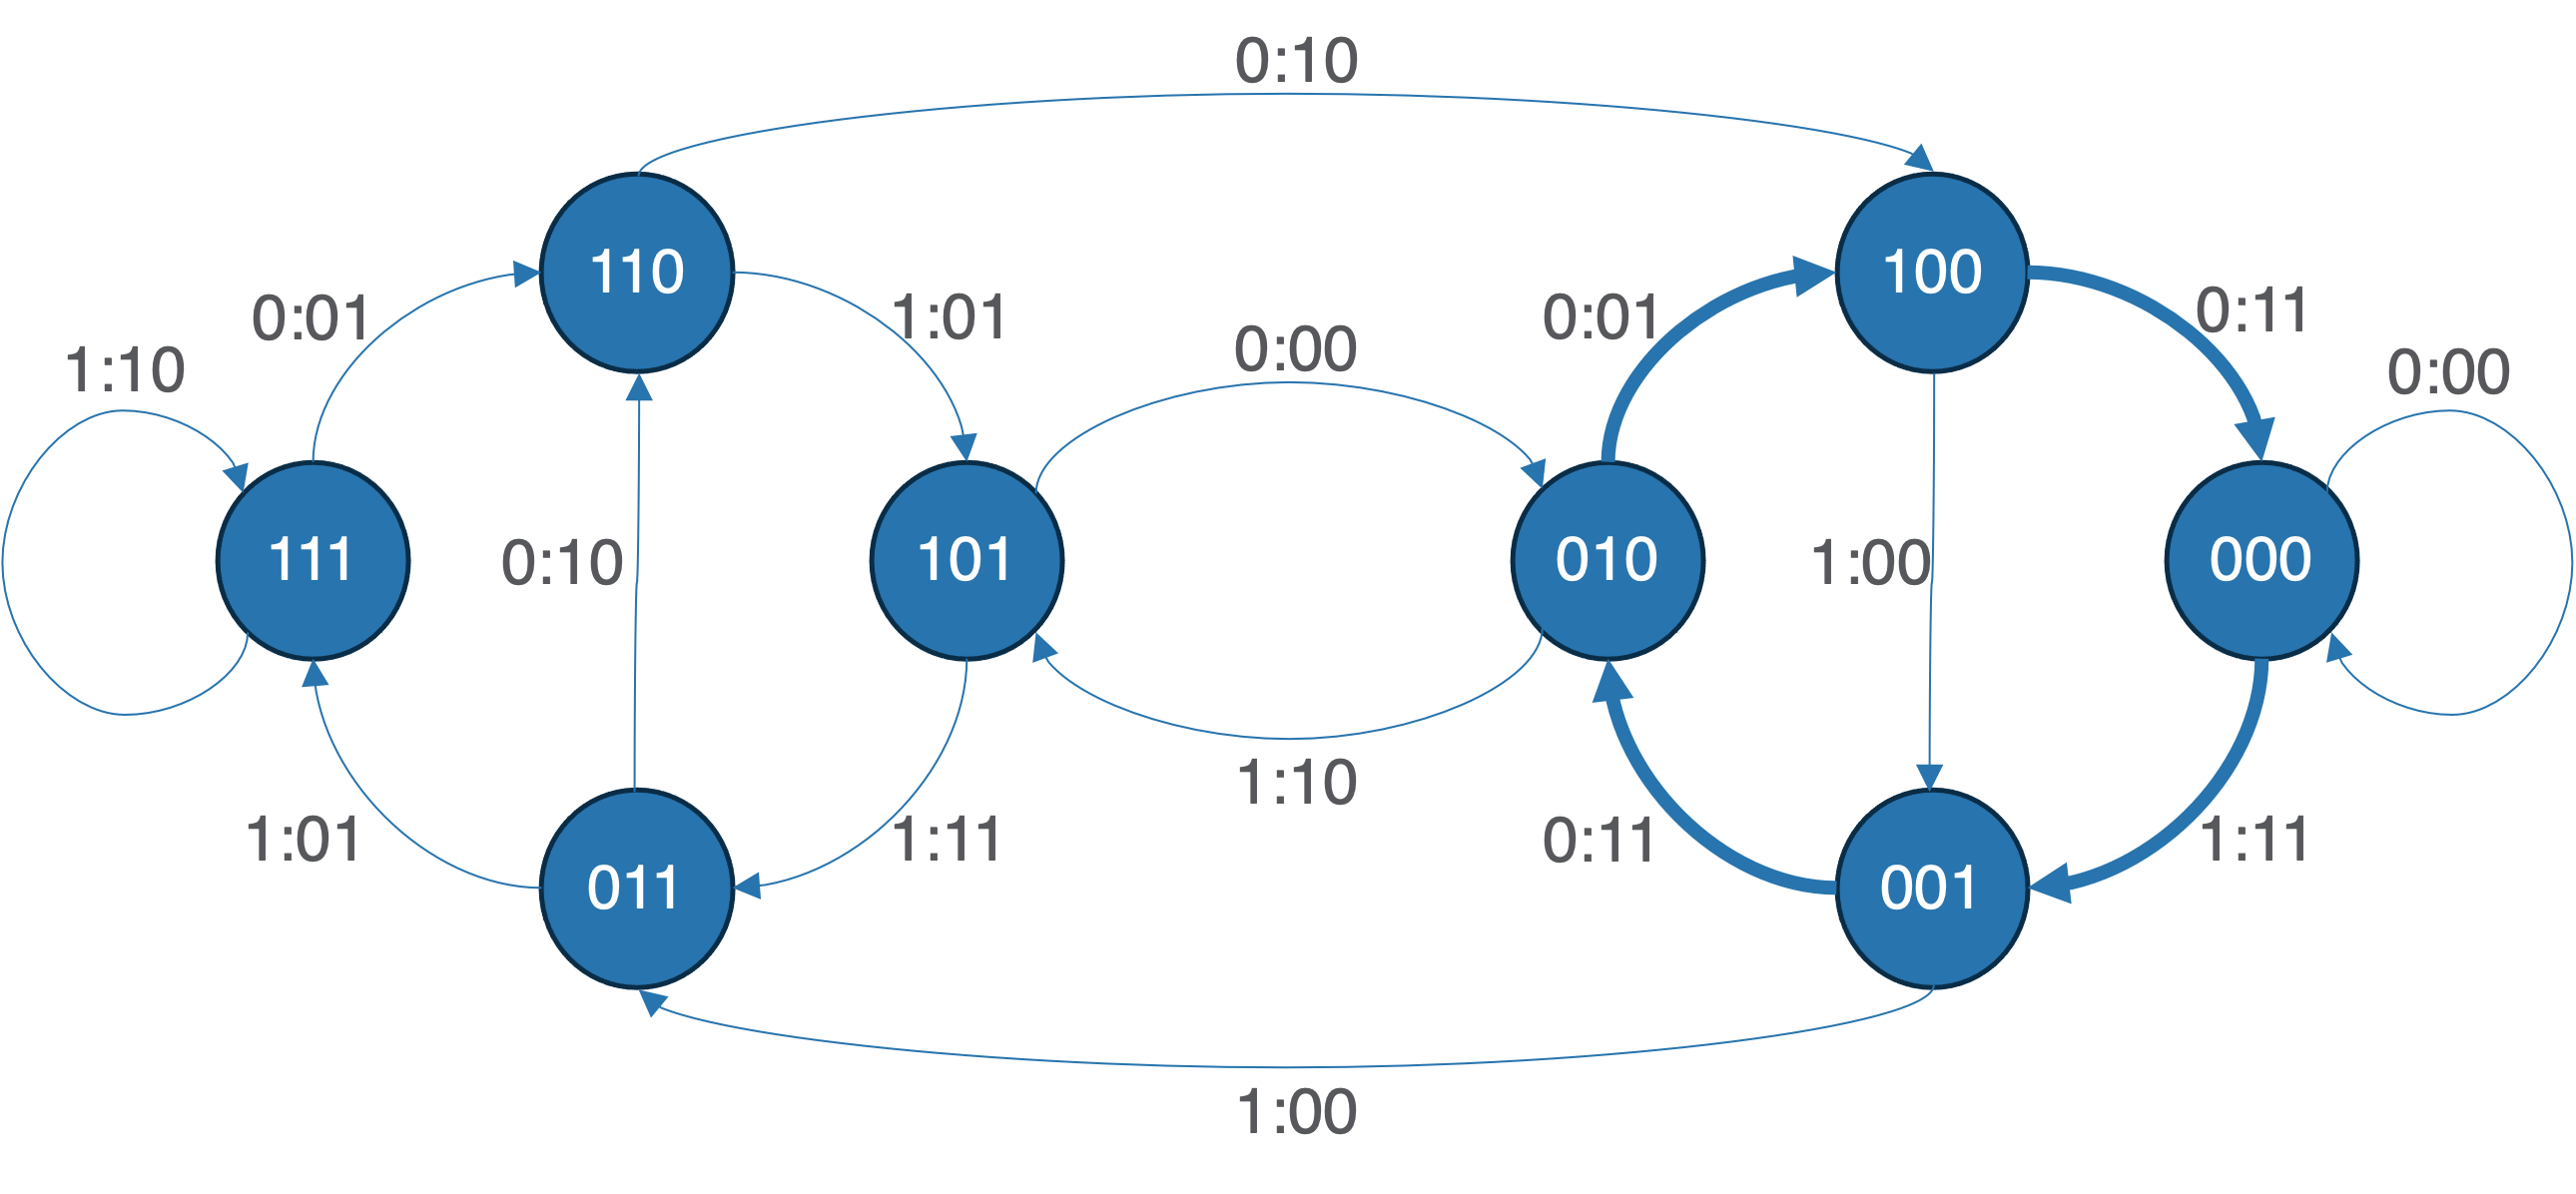
\includegraphics[height=15em]
{Figures/convolutional_code_state_diagram.png}
\caption[State diagram interpretation of a convolutional code]
{State diagram interpretation of a convolutional code}
\label{Figure:Background:ConvolutionalCodeStateDiagram}
\end{figure}
%%%%%%%%%%%%%%%%%%%%%%%%%%%%%%%%%%%%%%%%%%%%%%%%%%%%%%%%%%%%%%%%%

Each state in this diagram represents the previous $N$ message bits, i.e every possibility the values stored in the $N$ memory elements can take. Each state transition then represents updating the cascaded memory elements after a new message bit has been encoded. In this paper we will use the convention where the MSB of the state is the oldest encoded message bit. 

With this formulation, each directed edge of the state diagram $(s, s')$ is a transition with a corresponding bit-encoding pair $(u, c = (c_1, \ldots, c_k))$ such that $s' = (s_2, \ldots, s_N, u)$ and $c(D)=u(D)G(D)$ where $u(D)$ is the polynomial of the sequence $(u, s_1, s_2, \ldots, s_N)$ **. 

Putting everything together, given a starting state and a sequence of message bits $u = (u_1, \ldots, u_T)$, there exists a unique sequence of directed edges (a graph walk) on the state diagram and the sequence of corresponding bit-encoding pairs give the encoding $c$ of $u$. Shown above is an example of a state diagram where each edge is labeled by its bit-encoding pair.

\subsection{Trellis Diagram Representation}

A trellis representation (\Figure~\fref{Figure:Background:ConvolutionalCodeTrellisDiagram}) is identical in nature to the state diagram, except now each state has a unique node for different time points. Mathematically, each directed edge of the trellis $(s, s')$ for $s, s' \in S = (s^t_1, \ldots, s^t_N) | s^t_i \in \{0,1\} \text{  and  } 0 \leq t \leq T$. All other statements of ** still apply, and thus we see a walk (now a path) in the trellis graph again corresponds to a unique message $u$ and encoding $c$.

One important thing to note is that the structure of every $N$ state trellis is the same, and for two $N$ state convolution encodes, the only differences lie in the bit-encoding pair given by $G(D)$. 

%%%%%%%%%%%%%%%%%%%%%%%%%%%%%%%%%%%%%%%%%%%%%%%%%%%%%%%%%%%%%%%%%
% FIGURE: BACKGROUND: Convolutional Encoder Trellis Diagram
\begin{figure}
\centering\CaptionFontSize
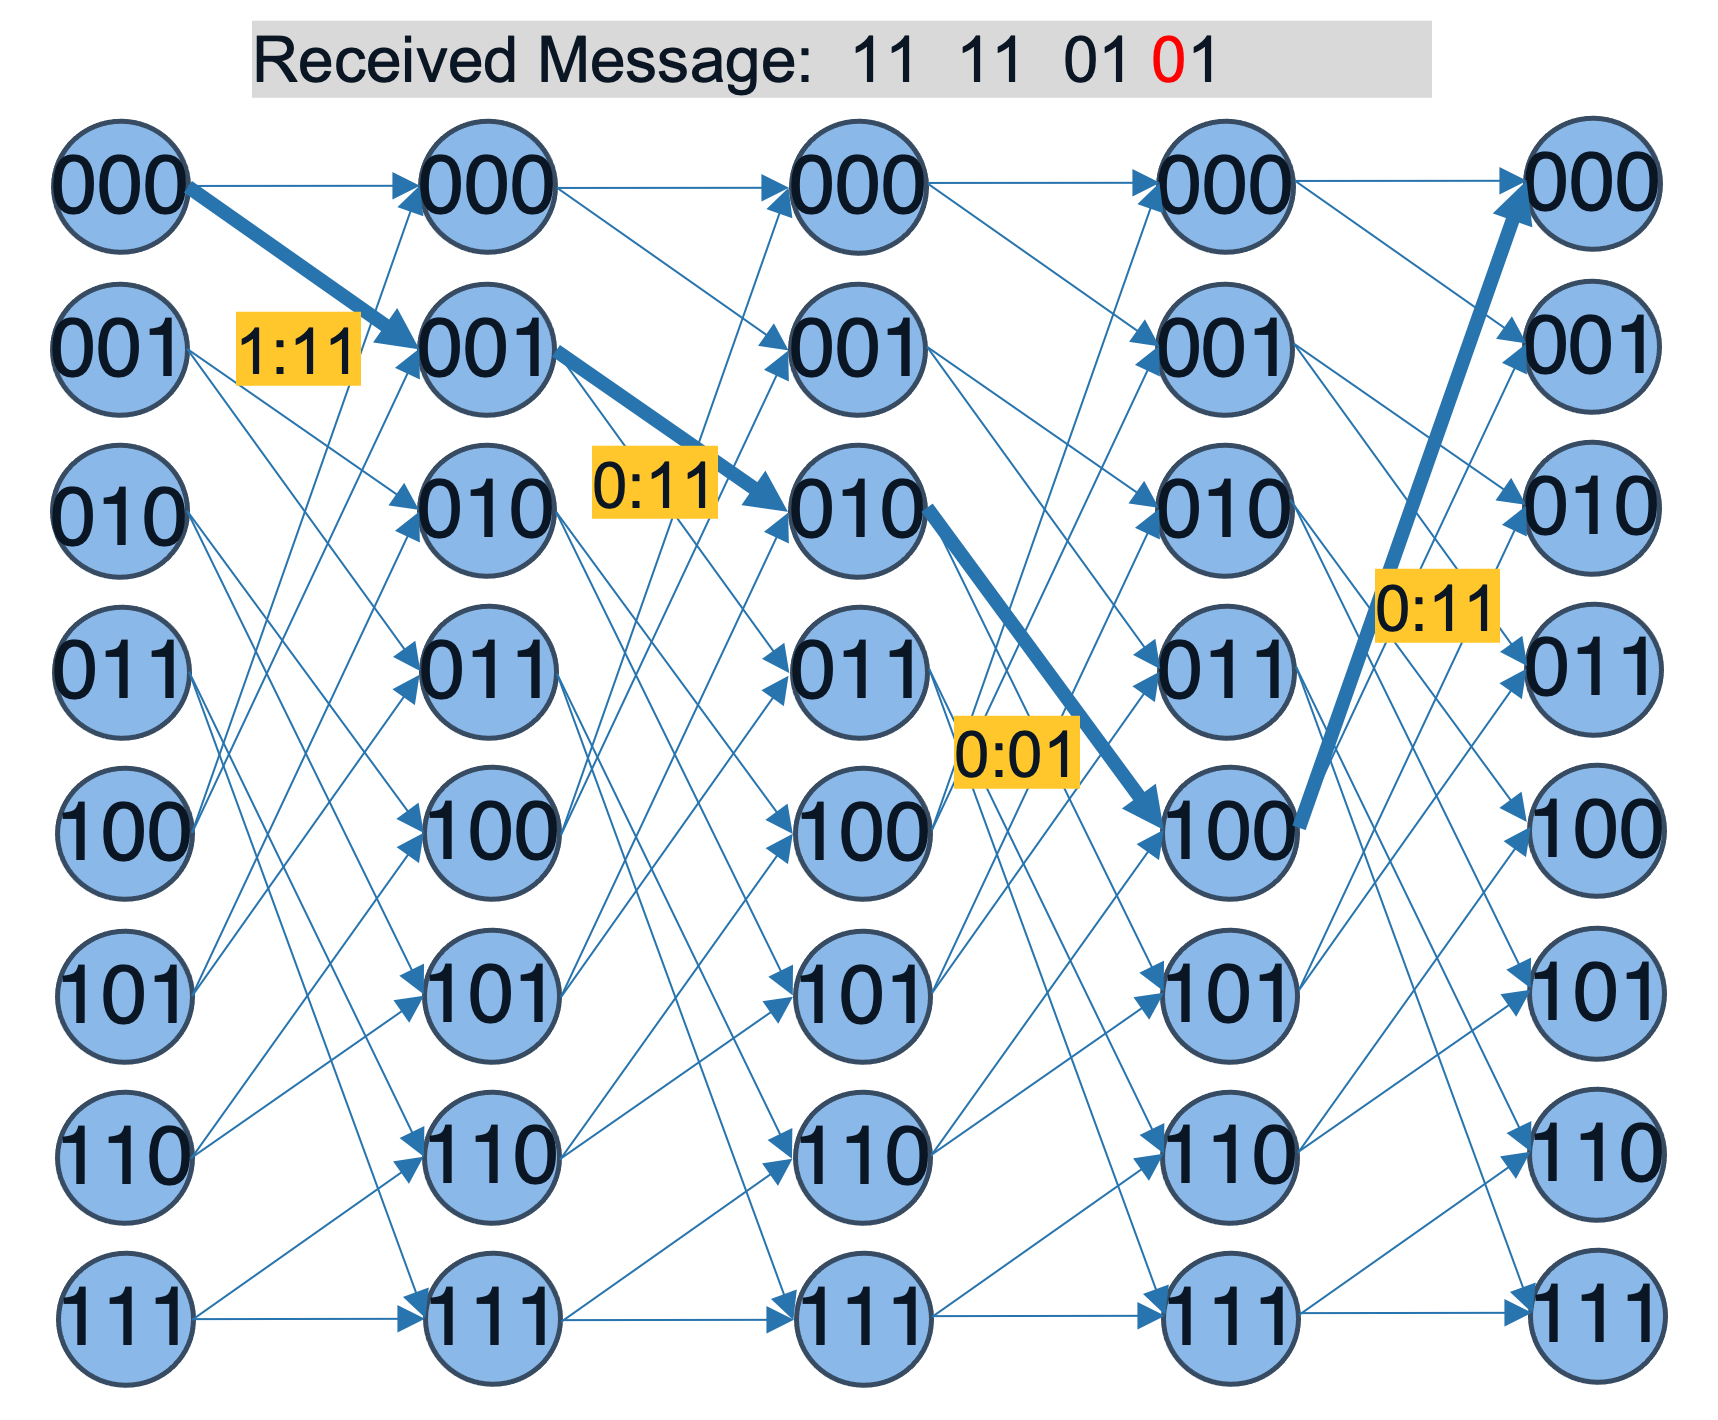
\includegraphics[height=20em]
{Figures/convolutional_code_trellis.png}
\caption[Trellis diagram interpretation of a convolutional code]
{Trellis diagram interpretation of a convolutional code}
\label{Figure:Background:ConvolutionalCodeTrellisDiagram}
\end{figure}
%%%%%%%%%%%%%%%%%%%%%%%%%%%%%%%%%%%%%%%%%%%%%%%%%%%%%%%%%%%%%%%%%

Henceforth we will denote space between the $i$th and $i+1$th column of the trellis as time points $t=i$. This is because each edge between columns represents the bit-encoding pairs, so if we split the encoded message into $T$ sections of length $k$ we can examine bit $t$ and its encodings in the trellis at time point $t$. 

\section{CRC \& Tail Biting Conditions}

Beyond the codes of interest being convolutional, we are particularly interested in CRC-aided Tail-Biting Convolutional Codes (TBCC). CRC and Tail-Biting conditions are both modifications to messages sent before encoding that streamline the transmission process. In this section we explain these modifications and the motivations behind using them.

Explanation
Cyclic Redundancy Check (CRC) is an additional form of protecting a transmitted message that appends a message with a string of bits that provides verification for the receiver that the message was received and decoded correctly. Typically, a system that includes a CRC aspect will have an agreed upon system of sending the transmitter a signal that acknowledges a successful transmission (ACK) and a signal for a failure (NACK); these are called Automatic Repeat Requests (ARQ). We call a code that has a CRC included in its encoding and decoding scheme a CRC-aided code. 

Another condition that we place on our convolutional codes is a tail biting (TB) condition. Typically, it is impractical to transmit one long continuous transmit message because it introduces complications in decoding. Instead messages are often split up and sent to the receiver in frames. In order for the decoder to decode a set of frames successfully, there must be a convention in place for the decoder to synchronize the decoding to start at the beginning of the frame. 

%%%%%%%%%%%%%%%%%%%%%%%%%%%%%%%%%%%%%%%%%%%%%%%%%%%%%%%%%%%%%%%%%
% FIGURE: BACKGROUND: CC Conditions
\begin{figure}
\centering\CaptionFontSize
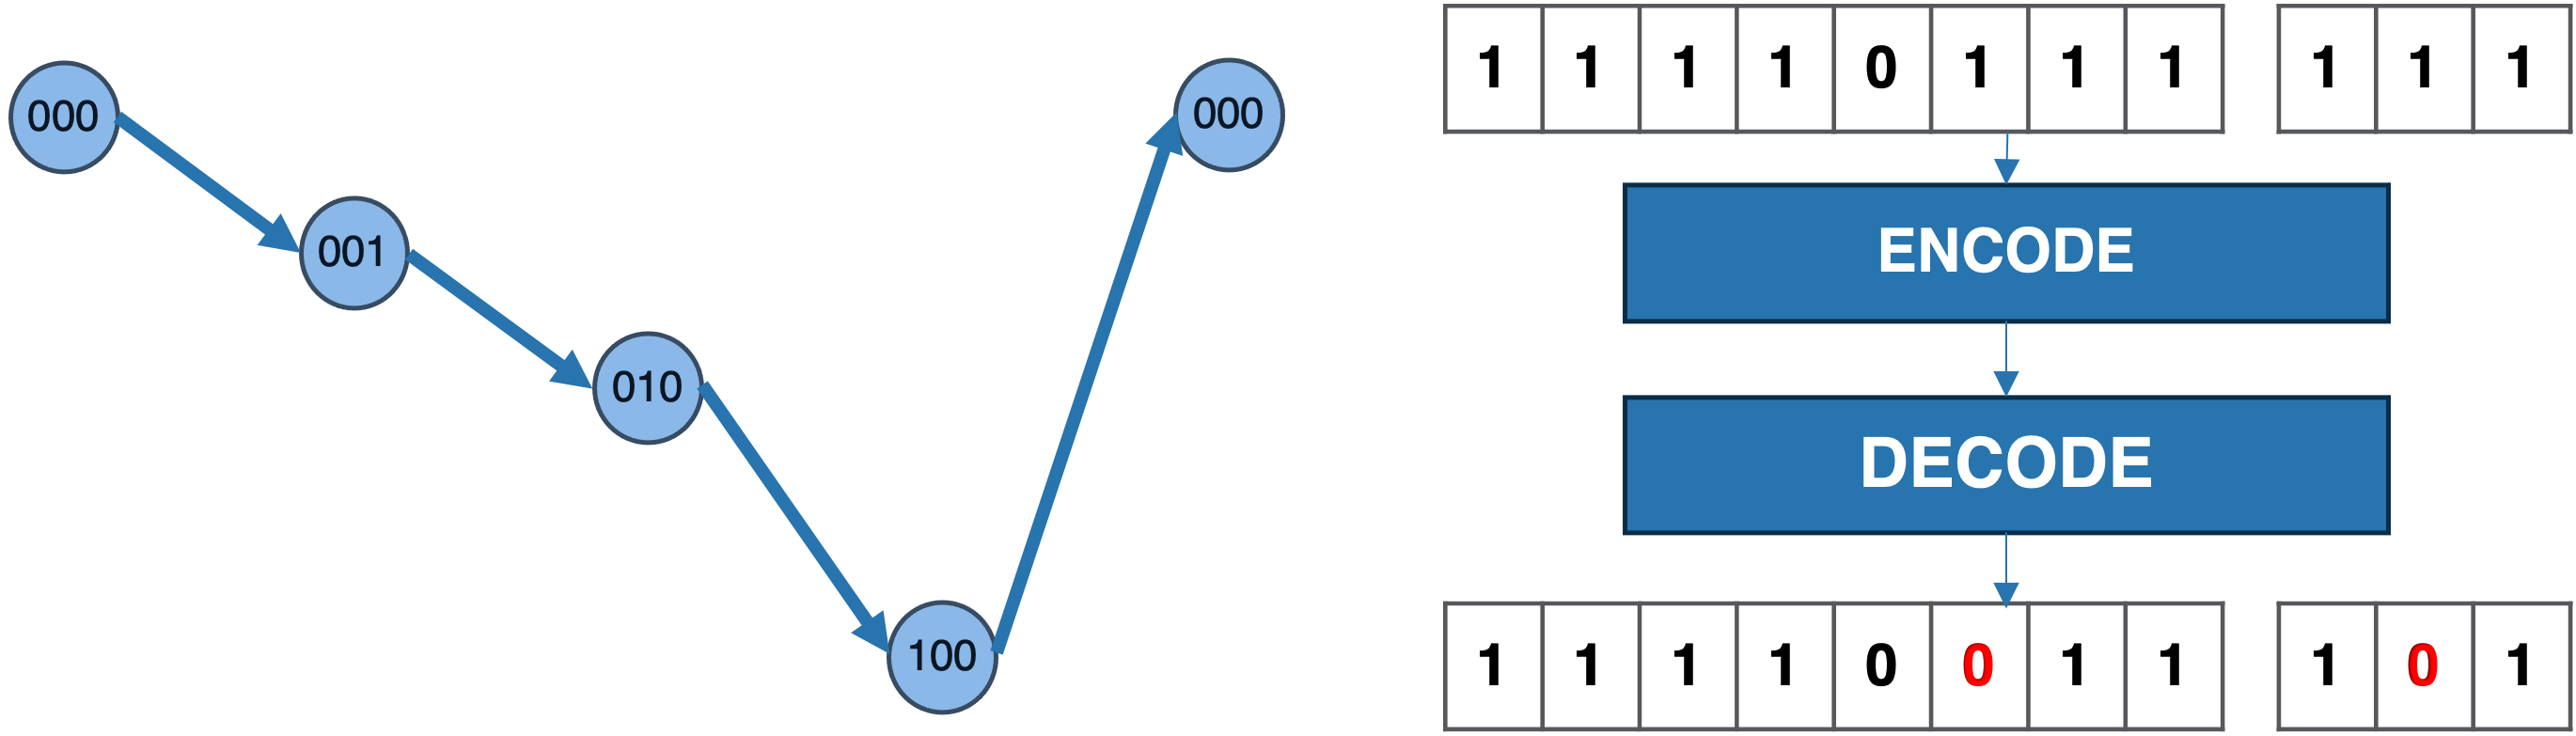
\includegraphics[width=\textwidth]
{Figures/code_conditions.png}
\caption[Visualization of CRC and Tail Biting Conditions]
{Visualization of CRC and Tail Biting Conditions. On the left is a picture of what a path in the trellis looks like when it passes the tail biting condition. On the right is an overview of how CRC is used to protect messages; the CRC portion is used to further provide error detection and correction in the original message.}
\label{Figure:Background:ConvolutionalCodeConditions}
\end{figure}
%%%%%%%%%%%%%%%%%%%%%%%%%%%%%%%%%%%%%%%%%%%%%%%%%%%%%%%%%%%%%%%%%
\TODO{fix image}
The tail biting condition is a method of frame synchronization where every frame of a sent message starts and terminates at the same state in encoding. Upon successful decoding and identification of a single frame, it then becomes easy for the decoder to identify all proceeding frames because frame length is predetermined. See \cite{Tailbiting} for more details.

\TODO{correct citing}

\section{Parallel List Viterbi Decoding (PLVD)}

Viterbi Decoding is a maximum likelihood (ML) approach to decoding a convolutional code using the Viterbi Algorithm (VA) to find the lowest metric path in the trellis with respect to the received message. We measure distance between to bit sequences with respect to a chosen metric; in this paper we choose something similar to the L2 norm, i.e the Euclidean distance between the two sequences.

As detailed in \cite{plvd}, both Serial List Viterbi Decoding (SLVD) and Parallel List Viterbi Decoding provide (PLVD) provide improved performance compared to VA, however we establish in the next section that PLVD has many algorithmic advantages that lend itself to hardware acceleration. 

\TODO{add citation}

The PLVD algorithm conventionally goes as follows. We iterate through time points starting at $t=0$. For each time point $t$, states will store a list of the $L$ paths of length $t$ with the lowest metric that end at that state $s$. For a path to have these properties, it is necessary that the path pass through the incoming edges of $s$ and thereby pass through the two states, at $t-1$ that share an edge with the $s$. WLOG let those states be $s^{t-1}_1$ and $s^{t-1}_2$ and let their respective stored lists be $l_1$ and $l_2$. To create the list of $L$ best paths at state $s$ we simply need to choose the $L$ paths with the best metric from $l_1 \cup l_2$ while taking into consideration the metric added along the incoming edges.

Formally we execute the following:

\begin{enumerate}
\item Since $t=0$ has no incoming edges, initialize and store a path starting at each state of length $0$ and with some initial metric (typically $0$).
\item For $1 \leq t \leq T$ do the following 
\begin{enumerate}
    \item For each state $s^t_i$, Let $e_1=(s^{t-1}_1, s^t_i)$ and $e_2=(s^{t-1}_2)$ be the incident edges on $s^t_i$ and $l_1$ and $l_2$ be the list of paths for $s^{t-1}_1$ and $s^{t-1}_2$.
    \item For $c$ being the received message from $t-1$ to $t$, choose the $L$ best paths from the set $\{l_1 + dist(e_1, c)\} \cup \{l_2 + dist(e_2, c)\}$ where the addition signifies adding the associated distance metric to all paths in $l_i$. 
    \item Store the chosen $L$ paths for each state.
\end{enumerate}
\item At $t = T$, we have a list of the $L$ lowest metric paths of length $T$. Out of all of these paths, choose the path with the lowest metric as our ML decoding of the received codeword.

\end{enumerate}

\subsection{Effect of TB and CRC}

In terms of execution of PLVD, the only thing that considerations for tail biting and CRC-aided codes change is our chosen path at the final $t=T$ state. Now, instead of simply choosing a path with the best metric, we must choose the path with the best metric that is tail biting and passes the CRC check. It is important to note that passing being tail biting and passing CRC are both strong conditions that drastically filter the list of valid paths at the final state. 






\chapter{Decoder HW Architecture}

\section{Introduction}
This section is an overview of the design for the hardware accelerated PLVD programming logic (PL) and explanations behind the optimizations implemented. The design is heavily based on Chester Hulse’s initial design \cite{ChesterPaper} who similarly details many of the following optimizations. This section will expand on Section IV of his paper and detail the specific improvements made to the original design. 

\TODO{Correct cite}

\section{Hardware Optimizations}

\subsection{Metric Computation}
In PLVD, the computation of edge metrics is heavily repeated and constitutes a large portion of the computational complexity of the algorithm. The following simplifications can be made to metric computations, drastically reducing the complexity of the algorithm. 

As described in the PLVD algorithm, at each time point t, we compare the k bits of received message at time point $t$ with the encodings given by every edge in the trellis at that $t$. 
For $R = (R_i, \ldots , R_k)$ and $C = (C_1, \ldots, C_k)$ with $R$ representing the log likelihoods of the received bits $X = (X_1, \ldots, X_k)$ (for BPSK $R_i = \log( \frac{P(U_i = 0 | X_i)}{P(U_i = 1 | X_i)})$ ) at some time point and $C$ being the correct encoding corresponding to that edge, we deem the ML code word to be one that minimizes the following
$$ \min_C \sum_i {(R_i - C_i)}^2 $$

This is akin to measuring the Euclidean distance, but we make the following simplifications that make the metric calculation much more realizable in hardware. The square terms can be disregarded ed since they are constant for each given time point. So we have the following
$$\min_C \sum_i -2 R_i C_i $$

Finally we can drop the -2 and maximize instead of minimize
$$\max_C \sum_i R_i C_i $$

This simplifies updating the edge metrics associated with a path at a time point to just adding the bit LLRs whose corresponding encoding bit is a $0$ and subtracting the LLRs who’s bit corresponds to a 1. An example is shown below

Ex. in a rate $\frac{1}{5}$ code we update path metric $m$ at time point $t$ with respect to received LLRs $R = (R_0 R_1 R_2 R_3 R_4)$ and edge weight (encoding) $11010$.
$$m = m - R_0 - R_1 + R_2 - R_3 + R_4$$

Furthermore, in this type of code, two edges that leave the same node necessarily have inverse encodings. Thus in the previous example, the other edge will have weight $00101$ and path metrics can be updated as
$$m = m + R_0 - R_1 - R_2 + R_3 - R_4$$

\subsection{Merge Sort}
Another expensive and repeated operation in PLVD is the storage and filtering of the list of best paths at each iteration. In particular, choosing the $L$ best paths from two unsorted lists of size $L$ is very difficult on a hardware level. To remedy this, our implementation stores the $L$ paths sorted by their metrics. The task is now simplified to choosing the $L$ best paths from two sorted lists of size $L$ and we proceed as follows:

\vspace{5pt}

Let $l_1, l_2$ be the two sorted lists of $L$ paths to be filtered. Repeat the following a total of $L$ times to obtain a sorted list $l'$ of the $L$ best paths.
\begin{enumerate}
    \item Compare the top elements of $l_1$ and $l_2$, and select the path $p$ with the better metric
    \item In $l'$, place $p$ directly after the most recently added element
    \item Remove $p$ from future consideration from $l_1$ or $l_2$ respectively
\end{enumerate}

%%%%%%%%%%%%%%%%%%%%%%%%%%%%%%%%%%%%%%%%%%%%%%%%%%%%%%%%%%%%%%%%%
% FIGURE: Decoder HW: Merge Sort
\begin{figure}
\centering\CaptionFontSize
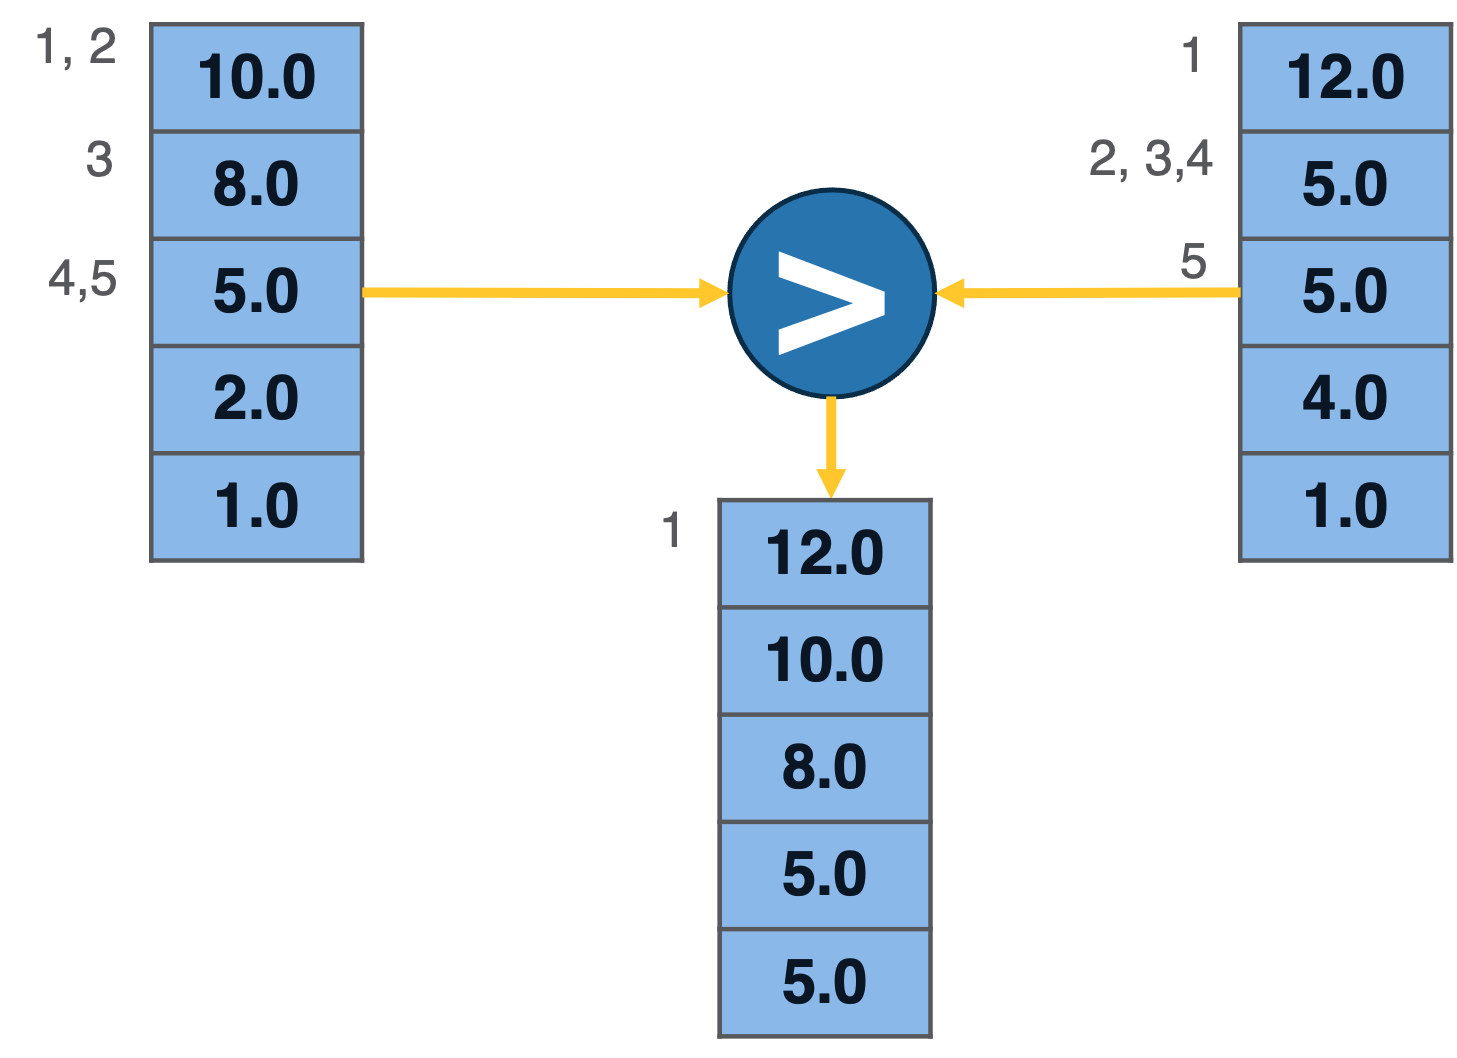
\includegraphics[height=15em]
{Figures/merge_sort.png}
\caption[Diagram detailing the merge sort sorting and storage of lists]
{Diagram detailing the merge sort sorting and storage of lists. Here $l_1$ and $l_2$ are shown with list lizes $L=5$. The numbers stored represent the path metrics (in reality there is more data stored in memeory) and the top values of the memory elements are always compared. Next to each entry is the iterations of the algorithm in which that value was examined for comparison.}
\label{Figure:DecoderHW:MergeSort}
\end{figure}
%%%%%%%%%%%%%%%%%%%%%%%%%%%%%%%%%%%%%%%%%%%%%%%%%%%%%%%%%%%%%%%%%

Note: from a data structures perspective, using a FIFO makes a lot of sense here, however, as we’ll see later, this actually ends up being more restrictive than we’d like.

\section{Hardware Architecture}
The overall architecture of the PLVD accelerator can be seen in \Figure~\fref{Figure:DecoderHW:OldArchitecture}. In this section we will discuss each module in detail. Aside from the LVA module, most others underwent minimal change from Hulse’s implementation \cite{ChesterPaper}, regardless, we explain for clarity.
\TODO{cite}

%%%%%%%%%%%%%%%%%%%%%%%%%%%%%%%%%%%%%%%%%%%%%%%%%%%%%%%%%%%%%%%%%
% FIGURE: Decoder HW: Old design architecture
\begin{figure}
\centering\CaptionFontSize
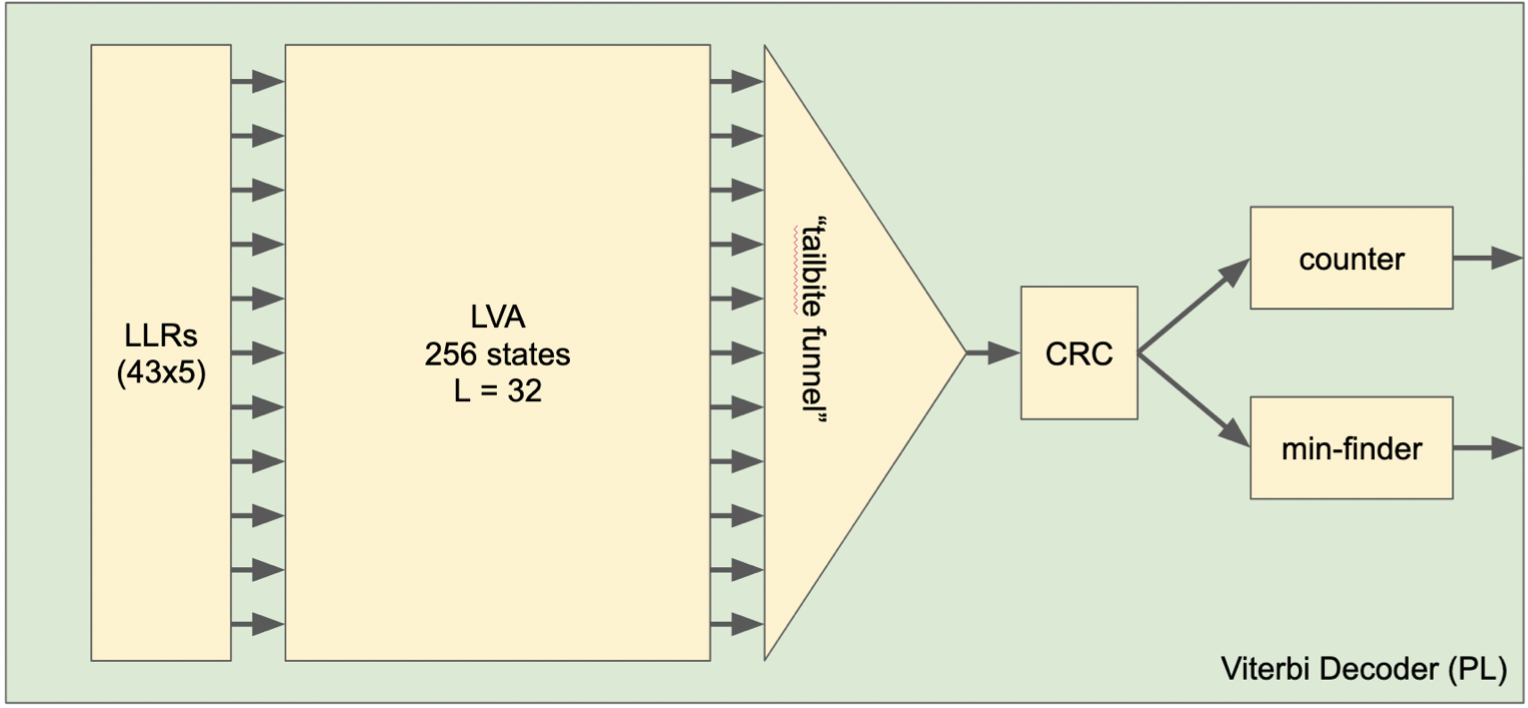
\includegraphics[height=15em]
{Figures/old_architecture.png}
\caption[Chester Hulse's design of FPGA PLVD]
{Chester Hulse's design of FPGA PLVD. Figure taken from \cite{ChesterPaper}}
\label{Figure:DecoderHW:OldArchitecture}
\end{figure}
%%%%%%%%%%%%%%%%%%%%%%%%%%%%%%%%%%%%%%%%%%%%%%%%%%%%%%%%%%%%%%%%%

The AMBA-AXI Stream interface is used to connect all modules where the data payloads are path objects as described below. AXI-Lite is used to handle fixed address memory access. 
\TODO{cite picture}
Input LLRs which represent the received code are stored in memory and serve as inputs for the LVA module. The LVA module runs PLVD as described above and outputs the L best paths through the trellis for each end state. The tail biting funnel module takes in parallel streams of paths and outputs a stream of paths that satisfy the TB condition. This stream is then passed through the CRC module that outputs the decodings that pass the CRC check. The decoding with the best metric is then chosen as the decoding of choice.

\subsection{Path Object}
This is the data structure used throughout the design that represents stores information about a path in the trellis. This is the data that is being written to memory and passed between modules via AXI. It holds 72 bits worth of data designed to maximize the width offered by BRAMs on a Xilinx ZCU106 board. Since we are investigating an 8 state, code with 43 transmitted bits, the data is structured as seen in \Figure~\fref{Figure:DecoderHW:PathObject}.

%%%%%%%%%%%%%%%%%%%%%%%%%%%%%%%%%%%%%%%%%%%%%%%%%%%%%%%%%%%%%%%%%
% FIGURE: Decoder HW: Path Object
\begin{figure}
\centering\CaptionFontSize
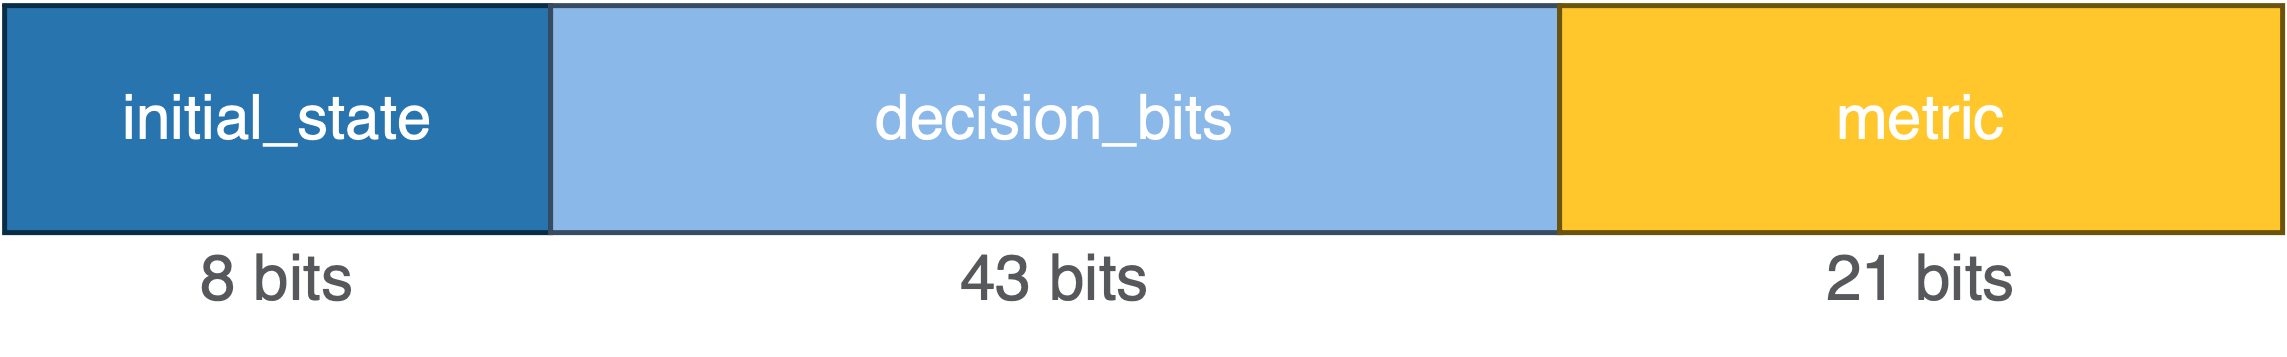
\includegraphics[width=\textwidth]
{Figures/path_object.png}
\caption[Diagram detailing the merge sort sorting and storage of lists]
{Diagram detailing the merge sort sorting and storage of lists. Here $l_1$ and $l_2$ are shown with list lizes $L=5$. The numbers stored represent the path metrics (in reality there is more data stored in memeory) and the top values of the memory elements are always compared. Next to each entry is the iterations of the algorithm in which that value was examined for comparison.}
\label{Figure:DecoderHW:PathObject}
\end{figure}
%%%%%%%%%%%%%%%%%%%%%%%%%%%%%%%%%%%%%%%%%%%%%%%%%%%%%%%%%%%%%%%%%

The “initial state” and “decision bits” elements give information on which path we are keeping track of while the “metric” element is the value that keeps track of the metric distance of the path with the received message. The size of the first two are fixed given the parameters of the convolutional code being transmitted, however, the number of bits used to calculate the metric was set to maximize the 72 bit structure of the BRAMs and can be changed as desired.

\subsection{LVA Module}
This module is the computational core of the decoder architecture which performs the PLVD algorithm. 
\subsubsection{Overview of Changes}
Hulse’s original design of the LVA core is in \Figure~\fref{Figure:DecoderHW:OldLVAModule}. Here, each state and edge in the state diagram has its own module; meaning at every time point, computations in steps 2a,b,c of the PLVD algorithm are done in parallel for every state; the design’s execution time depends only on the list size $L$ and the length of the code $T$. Furthermore, each state module uses two FIFO memory elements to store the incoming $L$ edge paths in order to implement the storage optimizations mentioned earlier. To implement these FIFO memory elements we ideally want to utilize high speed Programming Logic (PL) side Block Ram (BRAM).

%%%%%%%%%%%%%%%%%%%%%%%%%%%%%%%%%%%%%%%%%%%%%%%%%%%%%%%%%%%%%%%%%
% FIGURE: Decoder HW: Old LVA Module
\begin{figure}
\centering\CaptionFontSize
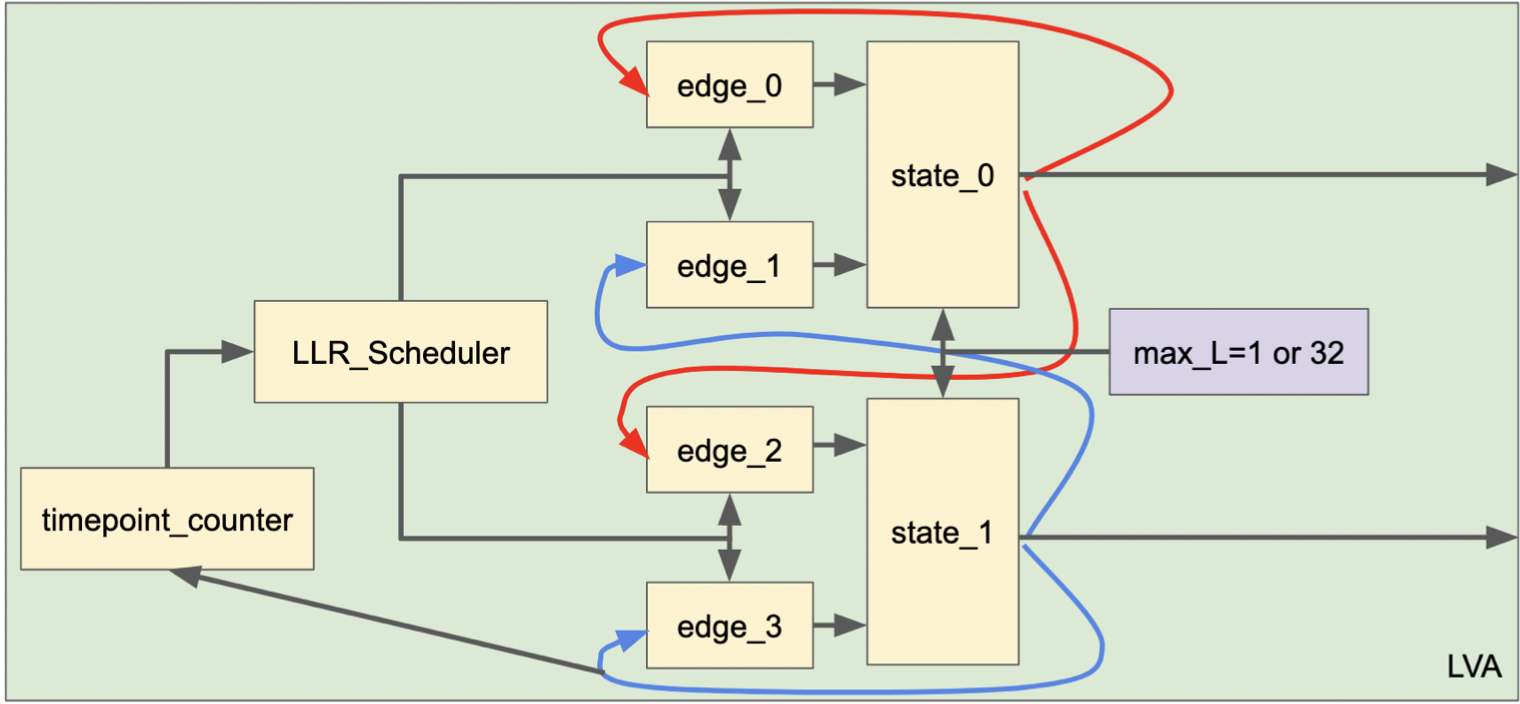
\includegraphics[height=15em]
{Figures/old_lva.png}
\caption[Chester Hulse's design of FPGA LVA]
{Chester Hulse's design of FPGA LVA. Figure taken from \cite{ChesterPaper}}
\label{Figure:DecoderHW:OldLVAModule}
\end{figure}
%%%%%%%%%%%%%%%%%%%%%%%%%%%%%%%%%%%%%%%%%%%%%%%%%%%%%%%%%%%%%%%%%
\TODO{Add cite}

While this design attempts to optimize the parallelism in the decoder, as Hulse mentions, for high state codes it draws too many resources. For example, in the $N=8$ ($S=256 \implies E=512$) case, the FPGA will attempt to synthesize 512 memory blocks which is more than most consumer FPGAs would contain. To synthesize this design on the ZCU106 Evaluation Board (which has 312 BRAM blocks) Distributed RAM was used to fill in the remaining ~200 memory elements (see \Figure~\fref{Figure:DecoderHW:OldUtilization}). Since Distributed RAM uses FPGA LUTs, this introduces routing and timing complications, forcing a lower clock speed, and takes too much space on the board to be reasonable. 

%%%%%%%%%%%%%%%%%%%%%%%%%%%%%%%%%%%%%%%%%%%%%%%%%%%%%%%%%%%%%%%%%
% FIGURE: Decoder HW: Old Design Utilization
\begin{figure}
\centering\CaptionFontSize
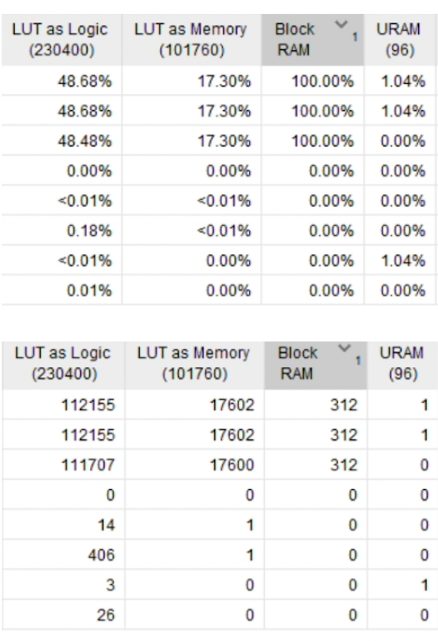
\includegraphics[height=20em]
{Figures/old_design_utilization.png}
\caption[Chester Hulse's design of FPGA LVA hardware utilization]
{Chester Hulse's design of FPGA LVA hardware utilization. Figure taken from \cite{ChesterPaper}}
\label{Figure:DecoderHW:OldUtilization}
\end{figure}
%%%%%%%%%%%%%%%%%%%%%%%%%%%%%%%%%%%%%%%%%%%%%%%%%%%%%%%%%%%%%%%%%
\TODO{cite}

%%%%%%%%%%%%%%%%%%%%%%%%%%%%%%%%%%%%%%%%%%%%%%%%%%%%%%%%%%%%%%%%%
% FIGURE: Decoder HW: FIFO Flushing
\begin{figure}
\centering\CaptionFontSize
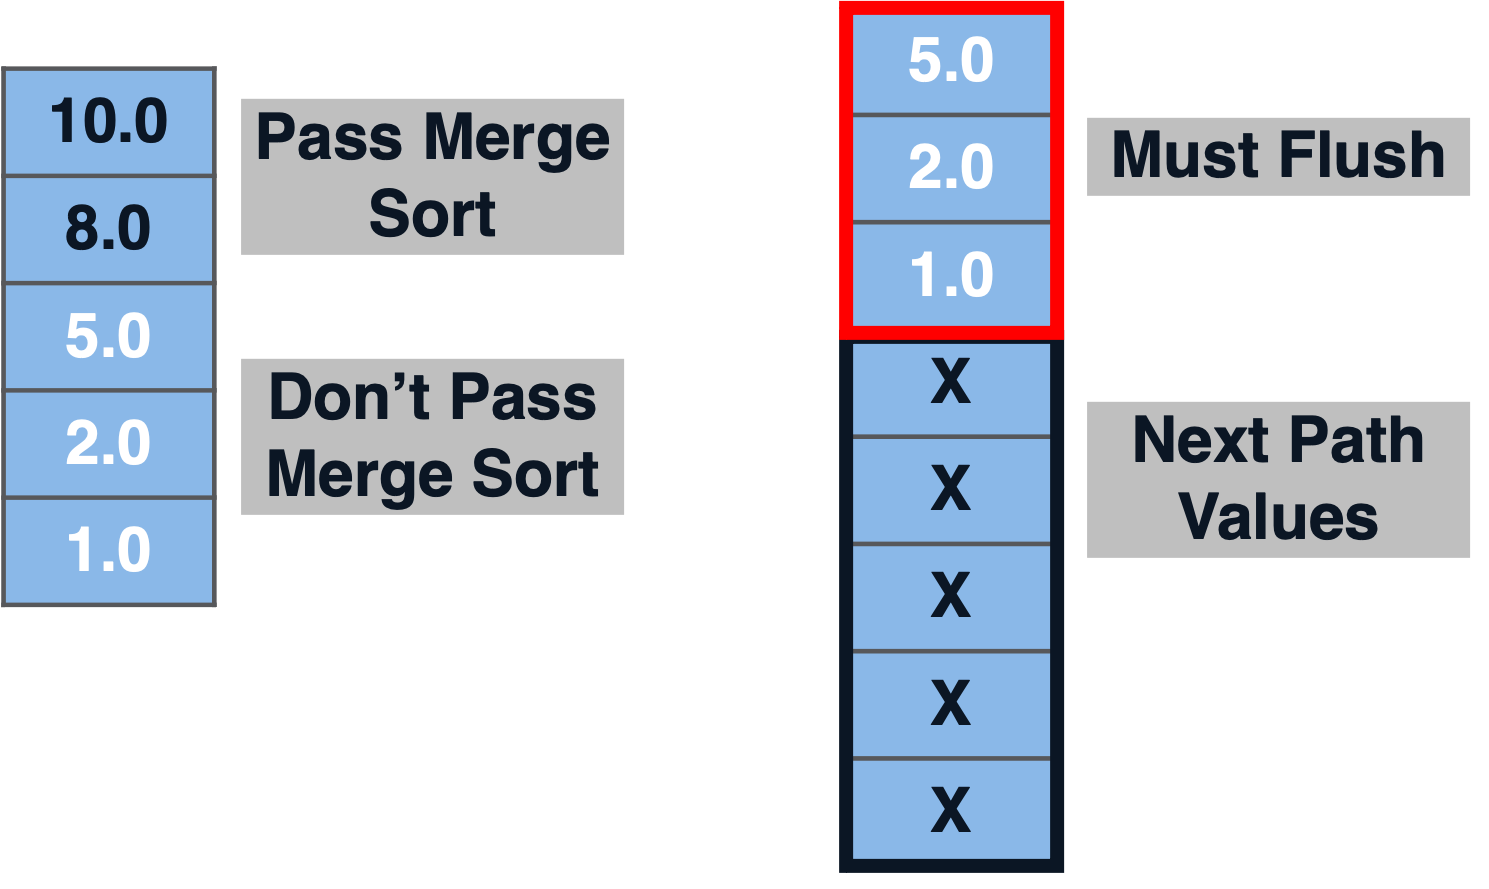
\includegraphics[height=15em]
{Figures/fifo_flush.png}
\caption[Example of FIFO flushing]
{Example of FIFO flushing.}
\label{Figure:DecoderHW:FifoFlushing}
\end{figure}
%%%%%%%%%%%%%%%%%%%%%%%%%%%%%%%%%%%%%%%%%%%%%%%%%%%%%%%%%%%%%%%%%

Additionally, implementing the list storage as a FIFO memory element introduces wasted cycles necessary to “flush” out old unused paths (see \Figure~\fref{Figure:DecoderHW:FifoFlushing}). In a best case scenario, after the $L$ best paths are chosen from the two lists of size $L$, there are still $\frac{L}{2}$ old paths that need to be flushed out of each FIFO before the decoder can move on to the next time point; at worst $L$ paths would need to be flushed.

To address these shortcomings Hulse proposes a change in his original design. Namely, introducing serialism to execution of PLVD per time point instead of attempting to do all state computations in parallel. The amount of parallelism in the implementation can be controlled by the number of BRAMs the user wants the decoder to utilize. In order to still decode high state codes and keep track of the same number of edge paths in the decoding process, each BRAM will have to store more than one edge list. This redesign also allows us to shift to a fixed memory structure instead of FIFO for better performance. The \Figure~\fref{Figure:DecoderHW:NewArchitecture} overviews the redesigned LVA architecture.

%%%%%%%%%%%%%%%%%%%%%%%%%%%%%%%%%%%%%%%%%%%%%%%%%%%%%%%%%%%%%%%%%
% FIGURE: Decoder HW: New Architecture
\begin{figure}
\centering\CaptionFontSize
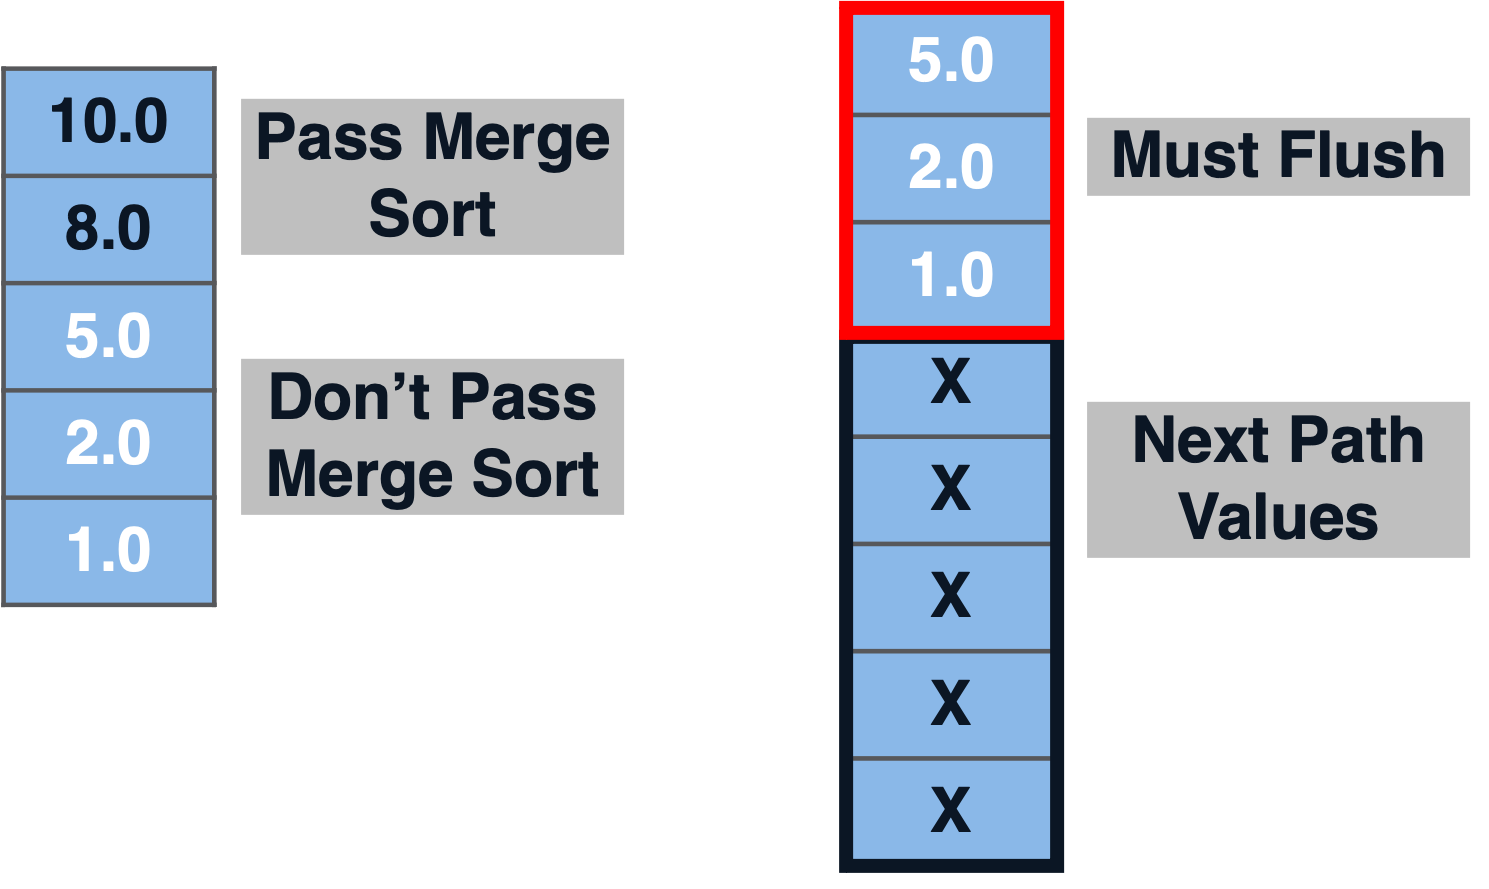
\includegraphics[height=15em]
{Figures/fifo_flush.png}
\caption[Proposed new hardware architecture]
{Proposed new hardware architecture.}
\label{Figure:DecoderHW:NewArchitecture}
\end{figure}
%%%%%%%%%%%%%%%%%%%%%%%%%%%%%%%%%%%%%%%%%%%%%%%%%%%%%%%%%%%%%%%%%
 
Henceforth we will use the parameters in to discuss the new design:
K = number of BRAMs allocated for decoder
S = number of states in the code
E = number of corresponding edges (2*S)

%%%%%%%%%%%%%%%%%%%%%%%%%%%%%%%%%%%%%%%%%%%%%%%%%%%%%%%%%%%%%%%%%
% TABLE: Decoder HW: Parameter Definitions
\begin{table}
\caption[Decoder HW chapter parameters]
{Chapter parameters}
\label{Table:Background:SymbolDefinitions}
\centering\CaptionFontSize
\begin{tabular}{c@{\hspace{1em}}l}
\toprule
Parameter & Definition
\\
\midrule
$K$ & number of BRAMs allocated for decoder
\\
$S$ & number of states in the code
\\
$E$ & number of corresponding edges (2*S)
\\

\bottomrule
\end{tabular}
\end{table}
%%%%%%%%%%%%%%%%%%%%%%%%%%%%%%%%%%%%%%%%%%%%%%%%%%%%%%%%%%%%%%%%%

Since we are no longer doing all state computations in parallel, we must have a system to determine which states we are processing and when. Since we have $K$ BRAMs we are limited to processing $K$ edges at any given moment, implying we can process $\frac{K}{2}$ states in parallel. If we denote a “state iteration” to be completing the computations for these $\frac{K}{2}$ states, then in order to complete all the computations for a given time point we would need $2*S/K = E/K$ state iterations. The new design keeps track of the state iteration using a counter which is utilized by the $\frac{K}{2}$ state and edge modules ( 1 edge module actually keeps track of 2 edges) as described below. Additionally, since we are using fixed memory, there are now bus modules that handle the flow of data in and out of the BRAMs that serve as $K$ multiplexers. 

\subsubsection{Memory and Memory Buses}
One benefit of the FIFO memory mechanism was that doing reads and writes at the same time would require half as much memory space compared to reading and writing from fixed memory. To implement this with fixed memory, the address space of each BRAM needs to be split into two sections. The first section contains the paths that were updated last time point which the decoder reads from. Those paths are used to calculate the metrics for paths in the current time point which are then stored in the second section. Once computations are finished and we move to the next time point, these sections in memory switch roles and the read section becomes the write section and vice versa.

The true bottleneck in the first design was over usage of BRAM blocks without utilizing their depth. This is why despite these changes increasing overall BRAM usage (by a factor of two), the flexibility of the design allows us to more fully utilize memory on board and process high order states.

However, in this design we encounter an interesting problem. Since each edge has a list of size $L$ paths associated with it at every time point, we must distribute the edges (i.e. the list of paths associated with each edge) such that each BRAM has $\frac{E}{K}$ edges associated with it. Furthermore, these edges need to be distributed in such a way that during execution there is always exactly one read and one write per cycle so that we maximize the utilization of the BRAMs available.

To accomplish this, there are two relevant axes of control,

\begin{enumerate}
    \item The choice of states we are processing in parallel
    \item The choice of which edges go into which BRAM
\end{enumerate}



To illustrate this challenge we consider a naive attempt at a solution. If for state $s$ in $[0, S-1]$, $e$ in $[0, E-1]$, and BRAM in $[0, K-1]$.

\begin{enumerate}
    \item We process states $\{0, 1, \ldots, K/2-1\}$, $\{K/2, K/2+1, \ldots, 2K/2-1\}$, $\ldots$ and $\{S-K/2, S-K/2+1 , \ldots, S-1\}$ in parallel.
    \item And we let edge $e$ be in in BRAM $e\%K (mod K)$
\end{enumerate}

Using this method to distribute edges, consider a case where $S = 8$, $E = 16$, and $K = 4$. We will have the following memory layout (\Figure~\fref{Figure:DecoderHW:NaiveMemory}) and execution order (\Figure~\fref{Figure:DecoderHW:NaiveOrdering}).

%%%%%%%%%%%%%%%%%%%%%%%%%%%%%%%%%%%%%%%%%%%%%%%%%%%%%%%%%%%%%%%%%
% FIGURE: Decoder HW: Naive Memory
\begin{figure}
\centering\CaptionFontSize
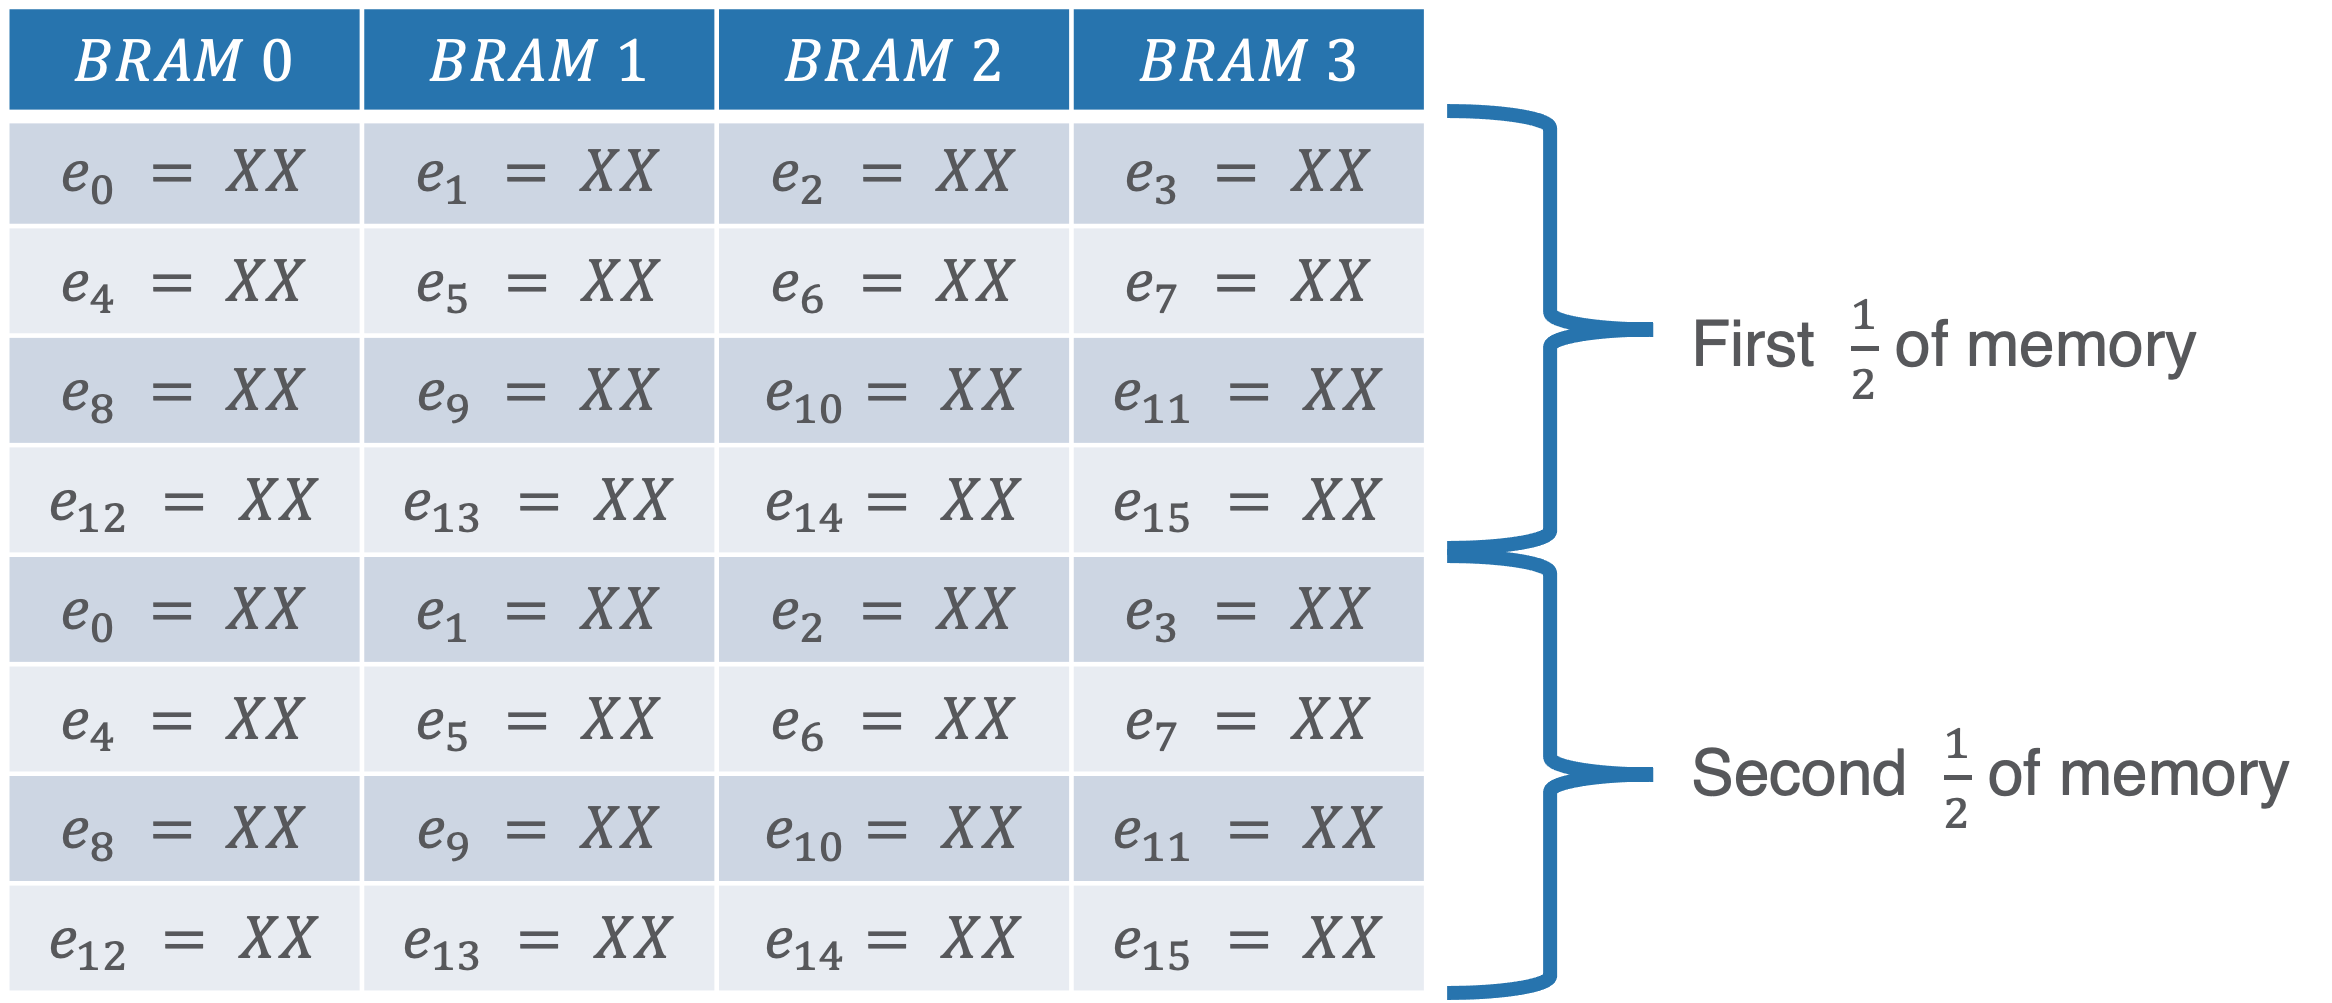
\includegraphics[height=15em]
{Figures/arb_fixed_mem.png}
\caption[Example of an arbitrary fixed memory structure]
{Example of an arbitrary fixed memory structure.}
\label{Figure:DecoderHW:NaiveMemory}
\end{figure}
%%%%%%%%%%%%%%%%%%%%%%%%%%%%%%%%%%%%%%%%%%%%%%%%%%%%%%%%%%%%%%%%%
%%%%%%%%%%%%%%%%%%%%%%%%%%%%%%%%%%%%%%%%%%%%%%%%%%%%%%%%%%%%%%%%%
% FIGURE: Decoder HW: Naive Ordering
\begin{figure}
\centering\CaptionFontSize
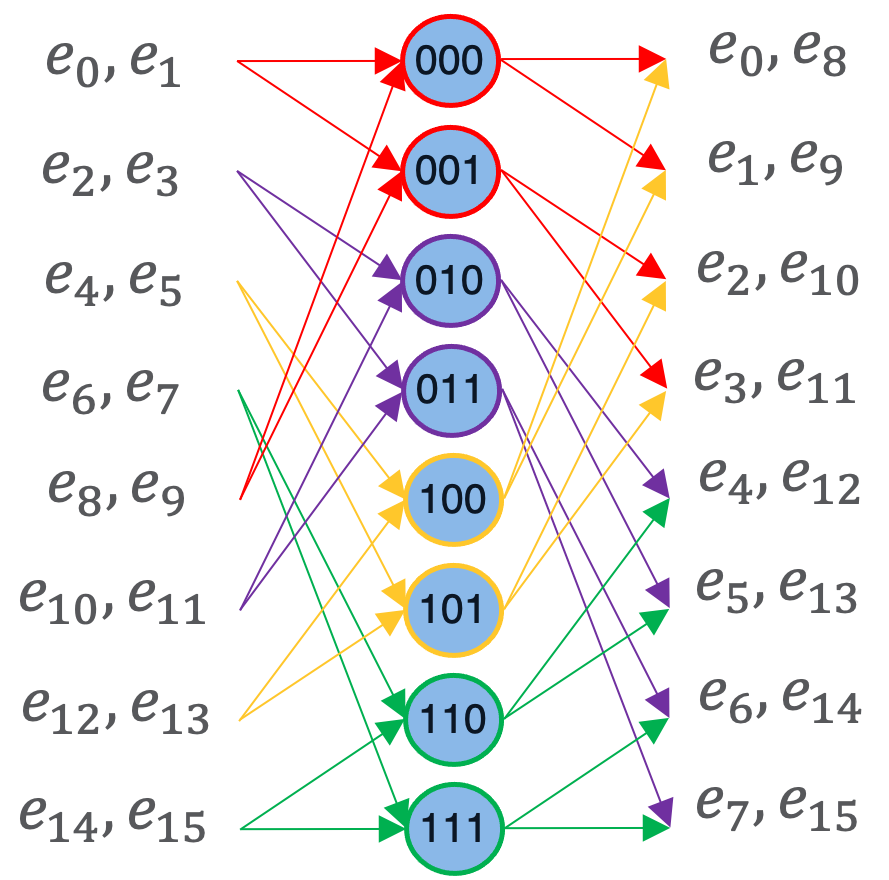
\includegraphics[height=15em]
{Figures/arb_state_ordering.png}
\caption[Example of an arbitrary execution ordering of states]
{Example of an arbitrary execution ordering of states. The execution ordering according to the naive solution would be red $\implies$ purple $\implies$ yellow $\implies$ green}
\label{Figure:DecoderHW:NaiveOrdering}
\end{figure}
%%%%%%%%%%%%%%%%%%%%%%%%%%%%%%%%%%%%%%%%%%%%%%%%%%%%%%%%%%%%%%%%%
In the first “state iteration” of executing the algorithm, we see that since $s_0$ and $s_1$ are being processed, that means that the decoder must read $e_0$, $e_1$, $e_8$, and $e_9$ from memory. However, based on the above memory layout, we must read from BRAM0 and BRAM1 twice and BRAM2 and BRAM3 are left unread. Thus we will inevitably waste cycles by waiting to do two reads, and are letting resources run idle.

Our solution fixes (1) to be the same as in the naive solution, but finds an adequate (2) that allows us to read and write with every BRAM every cycle. 

The solution, interestingly enough, was inspired from the very basics of encoding theory. If we consider each BRAM to have a particular ID represented in binary, then each of the K BRAMs would have a $\log_2(K) = k$ (different $k$ than rate $1/k$) long bit sequence ID. Using this formulation, the problem is redefined as associating each edge with a $k$ bit sequence such that if edges have the same bit sequence they don't share the same read/write state iteration. This association of edges to bits is effectively equivalent to finding a convolutional encoding, and thus we simply need to find a generator polynomial that satisfies the condition. With this realization, testing different strategies to determine a valid (2) became much simpler, and eventually we narrowed down the following encoding to be successful. 
$$G(D) = [ \sum_{n+1-k}^n D^i \quad D^{k-2} \quad \cdots \quad D \quad 1] $$

To prove its validity we simply need to show that for any state iteration, the edges read from memory all come from a unique BRAM and likewise for the edges written to memory. To proceed we will utilize the following 3 lemmas derived from (1) in our solution and general trellis structure observations

\begin{Thm:Lemma}
Due to (1) for arbitrary state iteration $i$, there are $\frac{K}{2}$ states being processed and specifically they are $\{i*K/2, i* K/2+1, \ldots, (i+1)K/2-1\}$. Representing $s$ as a bit sequence $s = (s_1, s_2, \ldots, s_N)$, this implies that every state processed in state iteration $i$ has the same bits $s_1, \ldots, s_{N-k+1}$ (i.e upper $N-k+1$ bits) but unique bit sequence $(s_{N-k+2}, \ldots, s_N)$ (lower $k-1$ bits).
 \label{Thm:Lemma:DecoderHW:Lemma1}
\end{Thm:Lemma}

\begin{Thm:Lemma}
 the edges that are incoming into $s$ are $e_0 = (0, s_1, s_2, \ldots, s_N)$ and $e_1 = (1, s_1, s_2, \ldots, s_N)$.
 \label{Thm:Lemma:DecoderHW:Lemma2}
\end{Thm:Lemma}

\begin{Thm:Lemma}
For any state $s$ in the trellis with bit sequence $(s_1, s_2, \ldots, s_N)$, the outgoing edges are $e_0 = (s_1, s_2, \ldots, s_N, 0)$ and $e_1 = (s_1, s_2, \ldots, s_N, 1)$
\label{Thm:Lemma:DecoderHW:Lemma3}
\end{Thm:Lemma}

\begin{Thm:Proposition}
The combination of (1) and (2) successfully label read edges and write edges such that every state iteration, there is exactly one read and one write from every BRAM.
\label{Thm:Proposition:DecoderHW:Prop1}
\end{Thm:Proposition}

\textbf{Proof of Proposition}

\underline{State Iteration Reads}: To prove our encoding successfully labels edges read at the same time differently, we split the set edges read from memory in an arbitrary state iteration into two cases: If two edges in set enter the same state and if they enter different states. 

In the case where two edges being read from memory are incoming to two on different states by \Lemma~\mref{Thm:Lemma:DecoderHW:Lemma2} $e^i = (e^i_1, s^i_1, s^i_2, \ldots, s^i_N)$ and $e^j = (e^j_1, s^j_1, s^j_2, \ldots, s^j_N)$. (2) necessarily gives the edges different encodings (BRAM IDs) since \Lemma~\mref{Thm:Lemma:DecoderHW:Lemma1} tells us the lower $k-1$ bits of s are distinct. In the other case, \Lemma~\mref{Thm:Lemma:DecoderHW:Lemma2} suggests that if two edges being read enter the same state $s$ then they must be of the form $e^i=(0, s_1, \ldots, s_N)$ and e$^j=(1, s_1, \ldots, s_N)$. Thus, the bottom $k-1$ bits of their encodings will be equivalent (properly), however, the evaluation of (2) to obtain the encoding MSB will be different since $(e^i_1) \neq e^j_1$ while $(e^i_2, \ldots, e^i_N-k+2) = (e^j_2, \ldots, e^j_N-k+2)$. In every case, the encoding procedure (2) produces different BRAM IDs. 

\underline{State Iteration Writes}: We take a similar approach to proving the encoding successfully labels write edges and split cases into edges exiting the different nodes and exiting the same node. 

\Lemma~\mref{Thm:Lemma:DecoderHW:Lemma3} implies two edges exiting the same node are of the form $e^i = (s_1, \ldots, s_N, 0)$ and $e^j = (s_1, \ldots, s_N, 1)$. Applying (2) to these edges, we immediately get different encodings since the LSB of the edges are different. For two edges exiting different states, \Lemma~\mref{Thm:Lemma:DecoderHW:Lemma3} implies $e^i = (s^i_1, \ldots, s^i_N, e^i_N)$ and $e^j = (s^j_1, \ldots, s^j_N, e^j_N)$. If $s^i_{N-k+2} = s^j_{N-k+2}$ then \Lemma~\mref{Thm:Lemma:DecoderHW:Lemma1} implies that the middle $k-2$ bits of $e^i$ and $e^j$’s encoding are different. If $s^i_{N-k+2} \neq s^j_N{-k+2}$ then the MSB of $e^i$ and $e^j$’s encoding are different since \Lemma~\mref{Thm:Lemma:DecoderHW:Lemma1} states that upper ${N-k+1}$ bits in the expressions (sum) and (sum) are the same. In every case, the encoding procedure (2) produces different BRAM IDs.

We have proven the solution (1) \& (2) solves the issue of BRAM to edge allocation, however, how about the location of edges within a particular BRAM? An interesting corollary to \Lemma~\mref{Thm:Lemma:DecoderHW:Lemma1} is that if two states $s^i$ and $s^j$ are processed in different state iterations, then their first $N-k+1$ bit sequences will be unique, i.e. $(s^i_1, \ldots, s^i_N-k+1) \neq (s^i_1, \ldots, s^i_{N-k+1})$. Thus we choose to start the list of arbitrary edges $e = (e_1, \ldots, e_N+1)$ at address $(e_1, \ldots, e_N-k+1, 0, \ldots, 0)$ where the number of inserted 0s is dependent on the maximum list size desired. This way, any edge processed in a different state iteration that shares a BRAM with e will necessarily have a different address for its list. Furthermore, edges within e’s state iteration might have the same address, but will be in different BRAMs. \Figure~\fref{Figure:DecoderHW:NewMemory} is an example of using this storage method for the K=4, S=8 case.

%%%%%%%%%%%%%%%%%%%%%%%%%%%%%%%%%%%%%%%%%%%%%%%%%%%%%%%%%%%%%%%%%
% FIGURE: Decoder HW: New Memory
\begin{figure}
\centering\CaptionFontSize
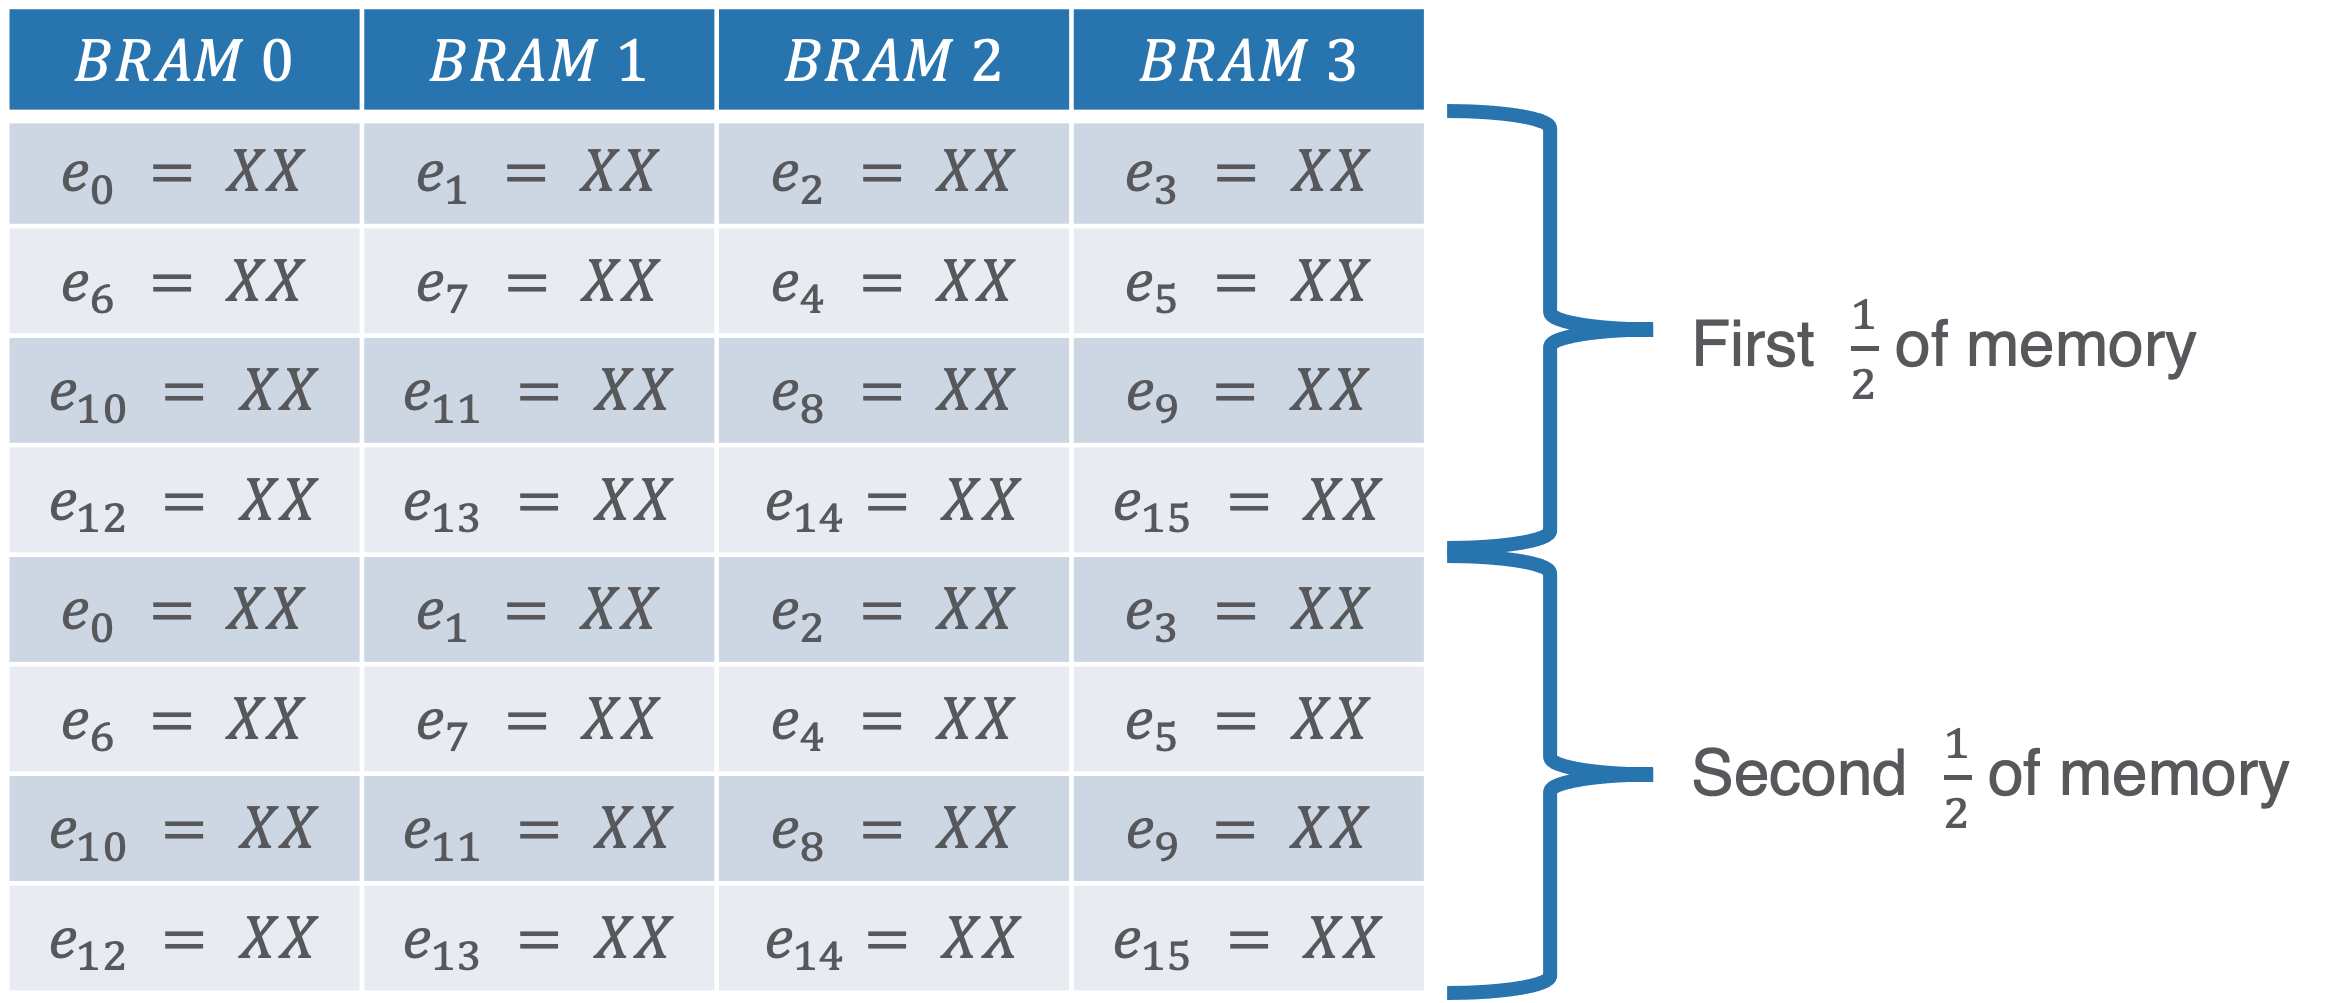
\includegraphics[height=15em]
{Figures/new_fixed_mem.png}
\caption[Example of new fixed memory structure]
{Example of new fixed memory structure.}
\label{Figure:DecoderHW:NewMemory}
\end{figure}
%%%%%%%%%%%%%%%%%%%%%%%%%%%%%%%%%%%%%%%%%%%%%%%%%%%%%%%%%%%%%%%%% 

Since we are using multiple addressable BRAMs to implement this design, a bus is necessary to serve as a multiplexor of BRAMs and handle the flow of data from memory to computation modules. Together, the memory and bus modules enable the decoder to efficiently read and write $K$ data streams as long as it’s provided with the proper BRAM IDs and addresses associated with the data being streamed.

We’ve established memory allocation for the list of paths in the decoder, this alteration somewhat forces changes in the state and edge modules from Hulse’s design.

\subsubsection{State Module}

Instead of instantiating $S$ state modules, LVA now instantiates $\frac{K}{2}$ modules each with a unique parameter STATE\_NUMBER that ranges from 0 to K/2-1. This parameter represents which “relative” state the module is processing each state iteration. As an input to the module are two AXI-LITE streams that correspond to the state’s two incoming edges. The iteration counter is also fed as an input (ITERATION) to the module and is used in conjunction with STATE\_NUMBER to calculate the base addresses of the two incoming lists. 
Using notation from the last section, \Lemma~\mref{Thm:Lemma:DecoderHW:Lemma1} implies that the states processed at ITERATION are s = (ITERATION, STATE\_NUMBER) where STATE\_NUMBER and ITERATION are respectively $k-1$ and $N-k+1$ bit sequences.

Thus, for the state module with parameter STATE\_NUMBER in ITERATION, \Lemma~\mref{Thm:Lemma:DecoderHW:Lemma2} and our methods for computing an edge’s BRAM ID and address give us simple hardware implementations that determine the base addresses of the lists required.

\begin{itemize}
    \item Top incoming edge:
    \begin{itemize}
        \item BRAM: G({0, ITERATION, STATE_NUMBER})
        \item address: (0, ITERATION>>1)<<$\log_2(Lmax)$
    \end{itemize}
    \item Bottom incoming edge:
        \begin{itemize}
        \item BRAM: G({1, ITERATION, STATE_NUMBER})
        \item address: (1, ITERATION>>1)<<$\log_2(Lmax)$
    \end{itemize}
\end{itemize}

Note that $G(D)$ is very efficient to do in hardware, only requiring $N-k+1$ XORs.

To execute the function of filtering the two incoming lists, each cycle the state module simply needs to read the data at the two computed base addresses, compare the two metrics, output the path with the better metric, and then increment the address that had that path by 1. This is repeated until either all valid paths have been read or $Lmax$ paths were outputted.

\subsubsection{Edge Module}
The changes to the edge modules are similar to the state module. Each of the $\frac{L}{2}$ edge modules use their unique STATE\_NUMBER and input ITERATION to calculate the base address of which two edges it is writing to. Its input is a stream of paths from its corresponding state module, and it outputs two AXI-LITE streams with updated path objects with metrics representing the state’s output edges. Furthermore, it inputs the LLRs associated with the received codeword for that time point.

The computations for an edge modules write locations are

\begin{itemize}
    \item Top incoming edge:
    \begin{itemize}
        \item BRAM: G({ITERATION, STATE_NUMBER, 0})
        \item address: (ITERATION)<<$\log_2(Lmax)$
    \end{itemize}
    \item Bottom incoming edge:
        \begin{itemize}
        \item BRAM: G({ITERATION, STATE_NUMBER, 1})
        \item address: (ITERATION)<<$\log_2(Lmax)$
    \end{itemize}
\end{itemize}

The edge module performs the metric calculations as detailed earlier by using STATE\_NUMBER and ITERATION to find the correct “mask” for one of the outgoing edges and using it to calculate the metric update $X$. The output path object for one of the edges will be the input path object with $X$ added to the metric, and the other output will subtract $X$ from the input path metric. These outputs will be AXI-LITE streams that write to the base addresses above in memory where every cycle the address increments by one.

\subsection{Projected Performance and Future Work}
Currently we are still in the process of implementing these changes to the design and running simulation/verification tests on the updated modules. Once complete, we aim to ensure these designs are synthesizable on board and compare resource utilization to the previous design and what is expected.

Since BRAMs used for memory is a user configurable parameter in our design ($K$), we expect BRAMs used to be $~K$. Thus, Distributed RAM instantiation should be 0 since they won't have to be used as BRAM substitutes anymore. Overall we also expect less arithmetic/logic since they correlate to the number of instantiated state and edge modules which scale with $K$. 

In terms of compute time, we expect the trellis propagation portion changing from finishing in $O(L*T)$ cycles to finishing in $O(2*S*L*T/K)$ cycles.

Once implemented and tested, this accelerated PLVD can be used as a computational core for simulating and implementing modifications to PLVD such as the work done by Jacob King \cite{king2023design}. Furthermore, accelerating PLVD allows us to compare its performance as a decoding scheme against other decoders such as SVLD and any future decoding algorithms.

\TODO{cite properly}



\chapter{Noise Generation}

\section{Introduction}
So far in this paper we have discussed an implementation of decoding CRC-aided TBCC on hardware that makes execution much faster than if done in software. However, suppose we wanted to simulate the performance of this code. This involves emulating an entire pipeline of encoding a message, distorting the transmission based on channel characteristics, and decoding. To retrieve bit and frame error rates of high SNR regimes, this emulation process must be repeated on the order of $10^15$ or more times. Despite the decoding portion of this process being accelerated, if the earlier steps in the simulation pipeline are done in software they will likely be a bottleneck for execution time. Thus we are motivated to hardware accelerate each step in this emulation process, of which, a hardware implementation of an additive white gaussian noise (AWGN) channel is critical. 

Below we detail a hardware module that generates an AWGN sample once per clock cycle. The implementation mimics the techniques detailed in \cite{noise_gen} which we summarize in the following section.


\section{Background}

Here we introduce the mathematical principles that allow this implementation to work as well as describe the challenges of implementing such principles in hardware.

\subsection{Box-Muller Method}
The Box-Muller transform is a transformation that generates two i.i.d normally distributed random variables using two i.i.d uniformly distributed random variables.

For $u_1, u_2 \sim U(0,1)$ and
$$f(u_1) = \sqrt{(- \ln(u_1))}$$
$$g_1(u_2) = \sqrt{2} \sin(2 \pi u_2)$$
$$g_2(u_2) = \sqrt{2} \cos(2 \pi u_2)$$

We see that RVs $x_1,x_2 \sim N(0,1)$ where

$$x_1=f(u_1)g_1(u_2)$$
$$x_2=f(u_1)g_2(u_2)$$



\subsection{HW Challenges}
The functions $f$, $g_1$, $g_2$ are all non-linear functions (f has particularly nonlinear regions around 0 and 1). Evaluation of these functions are critical to the accuracy of the generated distribution, thus, when designing hardware to implement these functions we aim to generate accurate approximations while minimizing the hardware footprint and complexity. A look-up table implementation is great for low precision applications, however, becomes spatially inefficient beyond a few bits since the table size will grow exponentially with input bits. Dividing the domain into uniform segments and approximating each segment with polynomial coefficients is another popular scheme, however, for highly non-linear functions is inaccurate. This approach segments the domain of the respective function non-uniformly, concentrating segments in areas with high non-linearity. To perform this in a way with simple hardware circuitry we utilize the binary nature of an address space and employ segments whose lengths vary by powers of two. 

\section{HW Design}

%%%%%%%%%%%%%%%%%%%%%%%%%%%%%%%%%%%%%%%%%%%%%%%%%%%%%%%%%%%%%%%%%
% FIGURE: Noise Generation: Noise Gen Architecture
\begin{figure}
\centering\CaptionFontSize
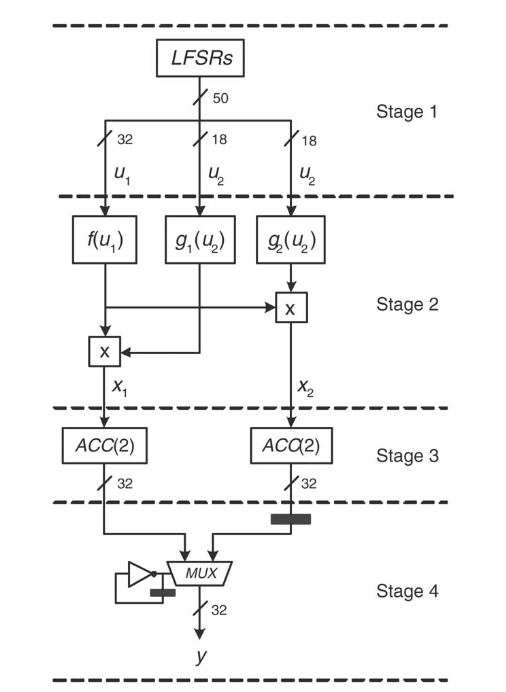
\includegraphics[height=20em]
{Figures/noise_gen_architecture.png}
\caption[Hardware architecture of an AWGN generator]
{Hardware architecture of an AWGN generator. Image taken from \cite{noise_gen}}
\label{Figure:NoiseGeneration:NoiseGenArchitecture}
\end{figure}
%%%%%%%%%%%%%%%%%%%%%%%%%%%%%%%%%%%%%%%%%%%%%%%%%%%%%%%%%%%%%%%%% 

The overall hardware architecture can be divided into four stages (see \Figure~\fref{Figure:NoiseGeneration:NoiseGenArchitecture}). Henceforth we discuss an implementation using 32 bits for precision. The only inputs driving this design are a clock, and the output is a 32 bit fixed point (4 integer bits and 28 fraction bits) representation of a normally distributed sample. 

\subsection{Stage I}

This stage generates the uniform random variables that get transformed using the approximated Box Muller method. This is implemented using Tausworthe generators \cite{noise_gen} which implement high periodicity uniform random samples using linear shift registers. These generators will output two 32 bit sequences that are interpreted as a fixed point float (all 32 bits fraction).

\subsection{Stage II}
In this stage, the Box Muller transform is applied to the two input RVs. The functions involved are segmented and approximated linearly. The output of these functions are then multiplied, generating two normally distributed samples.

%%%%%%%%%%%%%%%%%%%%%%%%%%%%%%%%%%%%%%%%%%%%%%%%%%%%%%%%%%%%%%%%%
% FIGURE: Noise Generation: F segmentation
\begin{figure}
\centering\CaptionFontSize
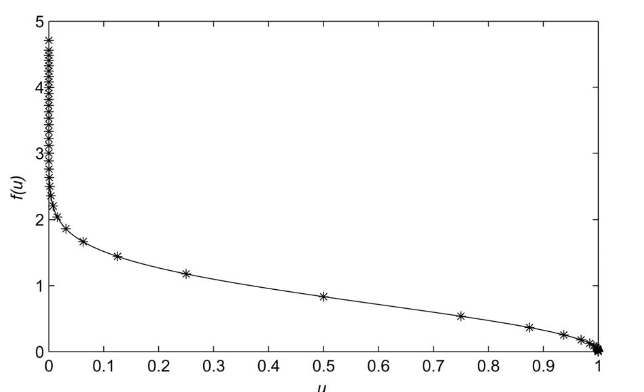
\includegraphics[height=15em]
{Figures/f_segmentation.png}
\caption[Non-uniform segmentation of f(u)]
{Non-uniform segmentation of f(u). Image taken from \cite{noise_gen}}
\label{Figure:NoiseGeneration:FSegmentation}
\end{figure}
%%%%%%%%%%%%%%%%%%%%%%%%%%%%%%%%%%%%%%%%%%%%%%%%%%%%%%%%%%%%%%%%% 
\TODO{cite}

The function f is segmented by placing segment boundaries at $0$, $2^{-n}$ for  $0 < n < 32$, $1-2^{-n}$ for $1<n<32$, and $1$ resulting in the domain being split into 62 segments. (\Figure~\fref{Figure:NoiseGeneration:FSegmentation})) is a graphical representation of this segmentation. Linear coefficients of these segments are stored in read only memory (ROM) addressed 0 to 61. To efficiently calculate an input’s segment and corresponding address in the ROM we employ a chain of OR and AND gates on the bits of the input as shown in an 8 bit example in \Figure~\fref{Figure:NoiseGeneration:AddressCalculator}). Each entry of the ROM has four values of interest: two base values and two scaling values for the first and zero-th order coefficients. Putting it all together, given an input $u$, $f(u)$ is evaluated by 

%%%%%%%%%%%%%%%%%%%%%%%%%%%%%%%%%%%%%%%%%%%%%%%%%%%%%%%%%%%%%%%%%
% FIGURE: Noise Generation: Address Calculator
\begin{figure}
\centering\CaptionFontSize
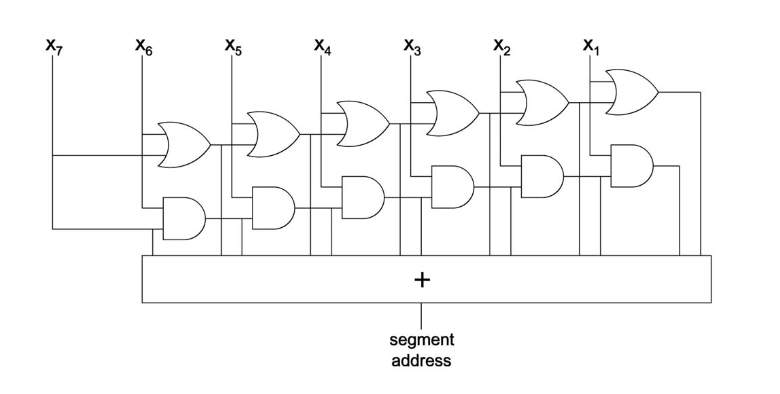
\includegraphics[height=15em]
{Figures/address_calculator.png}
\caption[8-bit example segment address calculator for non-uniform segmentation]
{8-bit example segment address calculator for non-uniform segmentation. Image taken from \cite{noise_gen}}
\label{Figure:NoiseGeneration:AddressCalculator}
\end{figure}
%%%%%%%%%%%%%%%%%%%%%%%%%%%%%%%%%%%%%%%%%%%%%%%%%%%%%%%%%%%%%%%%% 
\TODO{cite}

\begin{enumerate}
    \item Passing $u$ through the segment address calculator
    \item Reading the ROM at the address to obtain the linear coefficients of the corresponding segment: $c_{s1}$, $c_1$, $c_{s0}$, $c_0$ (calculated and flashed onto the board).
    \item Outputting the linear approximation $f(u) = 2^{(c_{s1})} (c_1 * u) + 2^{(c_{s0})} (c_0 )$
\end{enumerate}

%%%%%%%%%%%%%%%%%%%%%%%%%%%%%%%%%%%%%%%%%%%%%%%%%%%%%%%%%%%%%%%%%
% FIGURE: Noise Generation: G Symmetry
\begin{figure}
\centering\CaptionFontSize
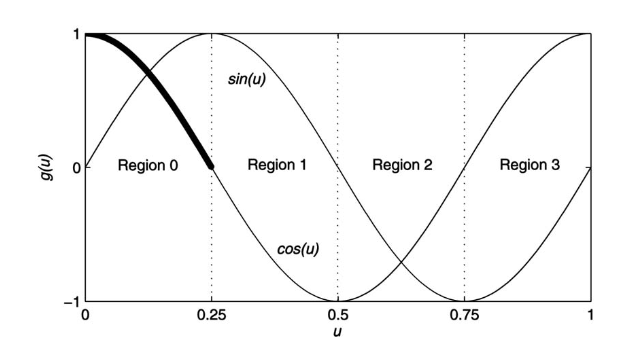
\includegraphics[height=15em]
{Figures/g_symm.png}
\caption[Illustration of the symmetry of $g_1$ and $g_2$]
{Illustration of the symmetry of $g_1$ and $g_2$. Image taken from \cite{noise_gen}}
\label{Figure:NoiseGeneration:GSymmetry}
\end{figure}
%%%%%%%%%%%%%%%%%%%%%%%%%%%%%%%%%%%%%%%%%%%%%%%%%%%%%%%%%%%%%%%%% 
\TODO{cite}

Due to symmetry of sin and cosine (\Figure~\fref{Figure:NoiseGeneration:GSymmetry})), functions $g_1$ and $g_2$ can both be evaluated just by performing approximations on the first $\frac{1}{4}$ of the domain of $g_2$. Below is a graphical representation of how this domain is segmented. Here we first uniformly segment the domain into 4 intervals and within each interval employ the same segmentation architecture described for $f$. For the first three intervals we segment into 6, and for the last segment we only segment into three (in architecture this corresponds to disconnecting certain branches from the adder). Aside from segmenting, everything pertaining to function evaluation is identical to $f$ except that the appropriate symmetry transformations are done to the linear approximation in order to obtain $g_1(u)$ and $g_2(u)$. We also drop the $\sqrt{2}$ multiplier in front of both functions due to the implementation of stage 3.

%%%%%%%%%%%%%%%%%%%%%%%%%%%%%%%%%%%%%%%%%%%%%%%%%%%%%%%%%%%%%%%%%
% FIGURE: Noise Generation: G Segmentation
\begin{figure}
\centering\CaptionFontSize
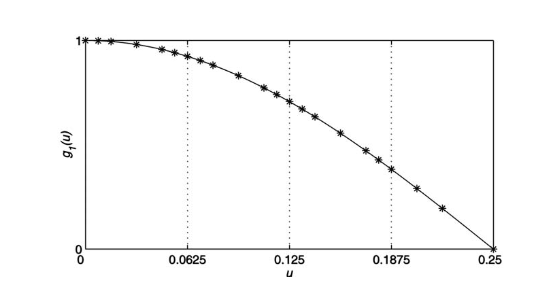
\includegraphics[height=15em]
{Figures/g_segmentation.png}
\caption[Non-uniform segmentation of Region 0 of $g$]
{Non-uniform segmentation of Region 0 of $g$. Image taken from \cite{noise_gen}}
\label{Figure:NoiseGeneration:GSegmentation}
\end{figure}
%%%%%%%%%%%%%%%%%%%%%%%%%%%%%%%%%%%%%%%%%%%%%%%%%%%%%%%%%%%%%%%%% 
\TODO{cite}

After having obtained approximated evaluations of $f(u_1)$, $g_1(u_2)$, and $g_2(u_2)$ we simply multiply the values together to obtain $x_1$ and $x_2$.

\subsection{Stage III}
In this stage we implement a small-scale application of the central limit theorem (CLT) and add successive outputs of the previous stage together. This is done in hardware using a size 2 accumulator for the $x_1$ outputs and another one for the x2 outputs. These will output the sum of the last two $x_1$ and $x_2$ samples generated which allows us to slightly employ CLT to introduce more normality in the samples while at the same time getting rid of need for the 
$\sqrt{2}$ multiplication in $g_1$ and $g_2$. Note that the output of this stage now generates two valid AWGN samples every other cycle; we fix this in stage 4.
\subsection{Stage IV}
This stage functions to alternate the outputs of stage 3 such that a sample is generated every cycle. This is done by simply buffering one output and then using a multiplexor to switch between the buffered output and the non-buffered output every cycle.

\section{Results and Future Work}

Running simulations of performance using this architecture, we see that it produces highly accurate AWGN samples. In our implementation, the approximations of the functions $f$, $g_1$, and $g_2$ have worst case absolute errors of 0.016, 0.0012, and 0.0012 respectively (see \Figure~\fref{Figure:NoiseGeneration:ApproximationError}). 

%%%%%%%%%%%%%%%%%%%%%%%%%%%%%%%%%%%%%%%%%%%%%%%%%%%%%%%%%%%%%%%%%
% FIGURE: Noise Generation: Approximation Error
\begin{figure}
\centering\CaptionFontSize
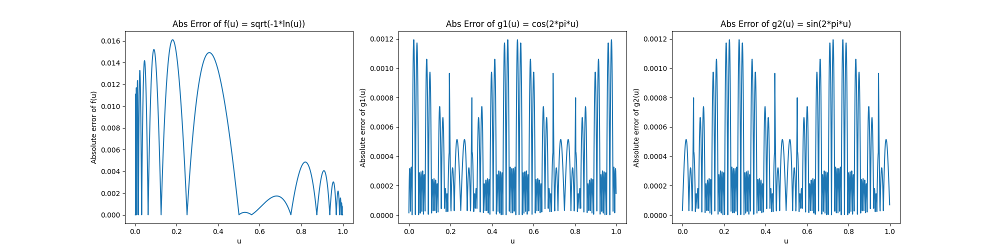
\includegraphics[width=\textwidth]
{Figures/approx_error.png}
\caption[Absolute error between hardware approximations and true value of $f$, $g_1$, and $g_2$]
{Absolute error between hardware approximations and true value of $f$, $g_1$, and $g_2$}
\label{Figure:NoiseGeneration:ApproximationError}
\end{figure}
%%%%%%%%%%%%%%%%%%%%%%%%%%%%%%%%%%%%%%%%%%%%%%%%%%%%%%%%%%%%%%%%% 

Furthermore, we are able to perform the Box-Muller method with high accuracy. \Figure~\fref{Figure:NoiseGeneration:UniformSamples} shows samples of a uniform distribution generated by the Tausworthe generators in stage 1 that get transformed into normally distributed samples at the output of stage 4 (\Figure~\fref{Figure:NoiseGeneration:NormalSamples}). These samples fit a normal distribution very well having only a 0.03 deviation from unit variance.

%%%%%%%%%%%%%%%%%%%%%%%%%%%%%%%%%%%%%%%%%%%%%%%%%%%%%%%%%%%%%%%%%
% FIGURE: Noise Generation: Uniform Samples
\begin{figure}
\centering\CaptionFontSize
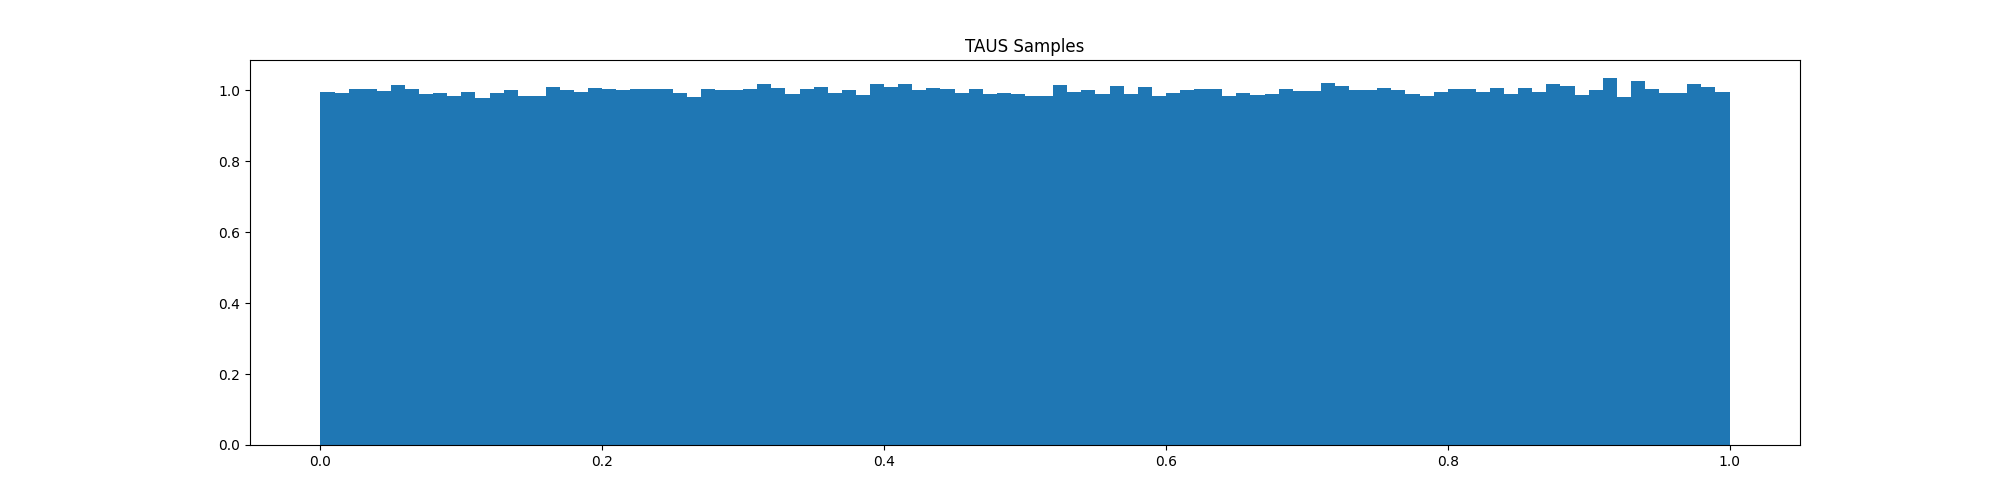
\includegraphics[width=\textwidth]
{Figures/uniform_dist.png}
\caption[Uniform random samples generated in hardware using a Tausworthe generator]
{Uniform random samples generated in hardware using a Tausworthe generator.}
\label{Figure:NoiseGeneration:UniformSamples}
\end{figure}
%%%%%%%%%%%%%%%%%%%%%%%%%%%%%%%%%%%%%%%%%%%%%%%%%%%%%%%%%%%%%%%%% 
%%%%%%%%%%%%%%%%%%%%%%%%%%%%%%%%%%%%%%%%%%%%%%%%%%%%%%%%%%%%%%%%%
% FIGURE: Noise Generation: Normal Samples
\begin{figure}
\centering\CaptionFontSize
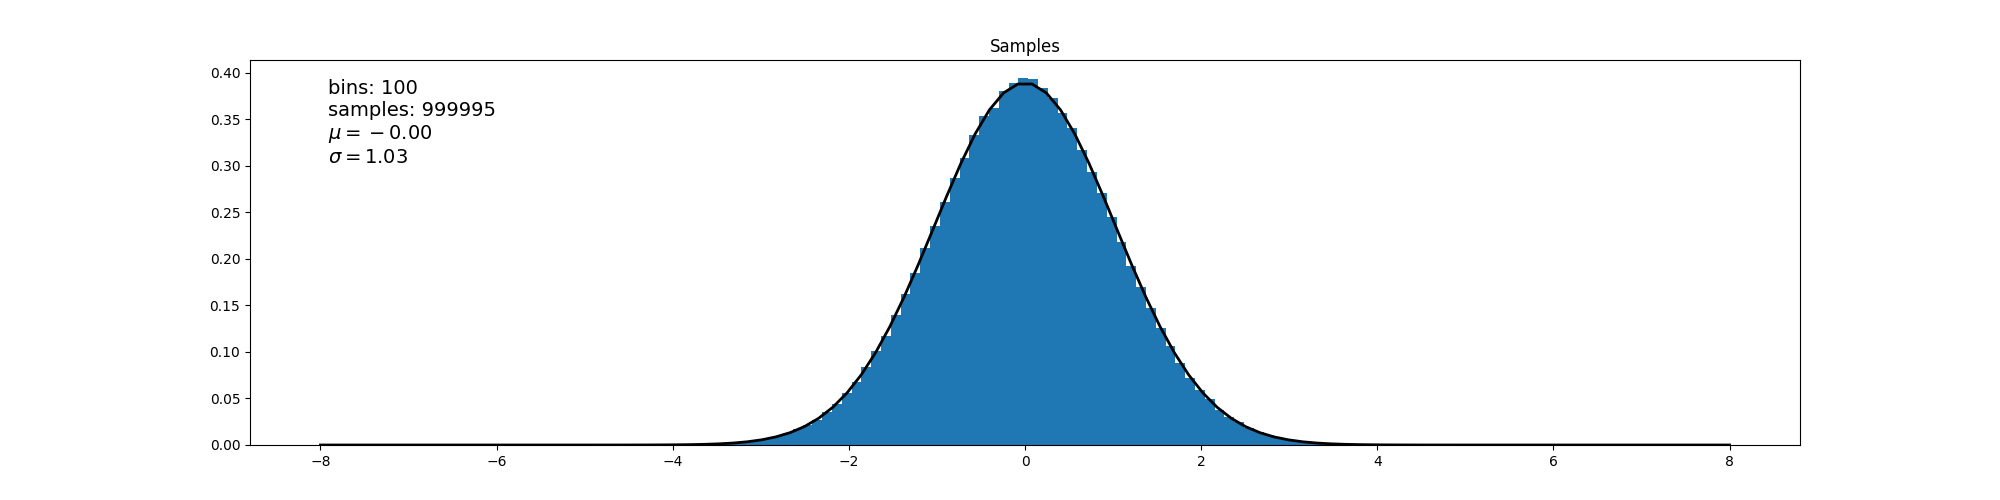
\includegraphics[width=\textwidth]
{Figures/normal_dist.png}
\caption[Normal random samples generated in hardware Box-Muller method implementation]
{Normal random samples generated in hardware Box-Muller method implementation}
\label{Figure:NoiseGeneration:NormalSamples}
\end{figure}
%%%%%%%%%%%%%%%%%%%%%%%%%%%%%%%%%%%%%%%%%%%%%%%%%%%%%%%%%%%%%%%%% 

Going forward we would like to examine the performance of this architecture at the tails of the distribution, an area that is quintessentially difficult to reproduce very well. Furthermore, there is room for improvement in terms of accuracy of the function evaluators. \cite{noise_gen} is able to reduce the absolute errors shown here by half and utilize less space on hardware, an effort that with more time can be accomplished with slight changes to the coefficient storage and calculation.



\chapter{Conclusion}
This thesis summarizes techniques to reduce the computational complexity of CRC-aided decoding of TBCCs on an FPGA as well as introduce optimizations to existing implementations of the PLVD decoding scheme. 

We first explain the motivation behind usage of CRC-aided TBCC and introduce techniques for interpreting encoding and decoding using the PLVD. We then introduce an existing implementation of PLVD and discuss the drawbacks of the design. We make modifications to this implementation that introduce parameterized resource usage and serialized execution. To do this we design an algorithm that manages memory allocation of edge lists in a way that is hardware synthesizable and efficient. 
In the final section, we showcase a hardware implementation of a AWGN generator that utilizes the Box-Muller transformation and efficient function segmentation to produce highly accurate AWGN samples. This hardware module can be utilized for simulating all kinds of codes on an FPGA as it is designed to be resource efficient.

With the accomplishments detailed in this paper, we are one step closer to realizing an end to end hardware implementation CRC-aided TBCC code transmission. We aim to finalize these implementations, execute simulations of performance, and compare results with other TBCC decoding schemes and theoretical performance bounds.

Work on this design is ongoing, and this thesis is intended to be a resource for those interested in the practical implementation of PLVD of CRC-aided TBCC on an FPGA as well as AWGN generation. 


%%%%%%%%%%%%%%%%%%%%%%%%%%%%%%%%%%%%%%%%%%%%%%%%%%%%%%%%%%%%%%%%%
%% BIBLIOGRAPHY.
%%%%%%%%%%%%%%%%%%%%%%%%%%%%%%%%%%%%%%%%%%%%%%%%%%%%%%%%%%%%%%%%%

\clearpage
\phantomsection
\addcontentsline{toc}{chapter}{Bibliography}

\bibliographystyle{IEEEtran} % IEEE bibliographic/citation style.
%\bibliography{IEEEabrv,Thesis}
\bibliography{IEEEfull,Thesis}


\end{document}
